\chapter{Molecular dynamics simulations predict hub residues involved in the allosteric transition of PKM2.}
\label{chapter:md}

\section{Introduction}
%
%
Allosteric ligand binding was shown in the previous two Chapters to affect changes to PKM2 activity by regulating the oligomeric state and the global conformational shape of the protein. Previous investigations have suggested that human PKM2 \cite{Morgan:2013aa}, and some of its orthologues \cite{Morgan:2010aa,Zhong:2017aa,Donovan:2016aa}, undergo a concerted rigid-body structural motion in response to FBP binding. In contrast, very little is known about the fine-grained molecular mechanism by which FBP and amino acids regulate PKM2; both in terms of the consequent energetic changes (either enthalpic or entropic) and the amino acid residues involved. Moreover, the structural resolution afforded by fluorescence spectroscopy and mass spectrometry measurements is limited. 
%
%
\\\\
%
%
An efficient strategy for probing allosteric regulation with sufficient temporal, spatial and energetic resolution, is the use of molecular dynamics (MD) simulations to model the conformational dynamics of proteins \cite{Durrant:2011aa,Guo:2016aa,Macpherson:2017aa}. Therefore, we sought to investigate the molecular mechanism of PKM2 allosteric regulation with a view towards identifying the specific protein residues, which are involved in propagating activating or inhibitory effects from distinct allosteric sites to the catalytic pocket, using MD simulations. In this Chapter, results are presented from a comprehensive study of the energetics and dynamics of monomeric and tetrameric PKM2 using computer simulations. Additionally, a novel computational method \textit{AlloHubMat} is described and applied towards extracting predicted allosteric hub residues in PKM2.

\clearpage


\section{Molecular dynamics simulations of PKM2 capture ligand-induced conformational changes}

To explore possible protein backbone conformational changes, elicited by allosteric ligand binding to PKM2, MD simulations of PKM2 were performed in the absence and in the presence of several allosteric ligands. Given that PKM2 exists as an equilibrium of oligomeric states (Section \ref{subsec:apo_pkm2_nms}), simulations of both monomeric and tetrameric protein were performed to investigate differences in the conformational dynamics between the two oligomers. Monomeric PKM2 was simulated in the apo-form (mPKM2$^{apo}$), bound to the endogenous inhibitor Phe (mPKM2$^{Phe}$), the endogenous activator FBP (mPKM2$^{FBP}$) and the exogenous small-molecule activator Tepp-46 (mPKM2$^{Tepp}$). Similarly, to investigate the dynamics involved in the ligand-induced conformational transition of PKM2 (Section \ref{subsec:fbp_ccsd}), simulations of tetrameric PKM2 were seeded from protein crystal structures in the apo-form (tPKM2$^{apo}$), bound to FBP (tPKM2$^{FBP}$), concurrently bound to serine and FBP (tPKM2$^{FBP+Ser}$) and bound to phenylalanine and FBP (tPKM2$^{FBP+Phe}$).


\subsection{An integration time step of 2 fs appropriately conserves the energy in monomeric PKM2 simulations}
Prior to production runs in the NPT ensemble, short 40 fs simulations of mPKM2$^{apo}$ were performed in the microcanonical (NVE) ensemble to evaluate the conservation of total energy of the system with integration time step sizes of 2 fs, 3 fs and 4 fs.The total energy fluctuations of the system were compared to those of the potential energy and the kinetic energy:
%
%
\begin{equation}
\Delta E = \sqrt{( E - \langle E \rangle )^2 }
\label{equ:energy_fluc}
\end{equation}
%
%
where $E$ is either the total, kinetic or potential energies of the system.
%
%
\\\\
%
%
Increasing the integration time step of the short NVE simulations resulted in a considerable increase in the amplitude of the fluctuations of the potential and kinetic energies (\textbf{Fig. \ref{fig:timestep}}). To reduce errors propagated from integrating the equations of motion, fluctuations of the total energy should be less than one-fifth of the fluctuations of the kinetic or the potential energies \cite{Winger:2009aa}. This criteria was not fulfilled for simulations using time steps larger than 2 fs (Table \ref{tab:timestep}), and so an integration time step of 2 fs was used in all subsequent simulations of monomeric and tetrameric PKM2.

%%% FIGURE
%
\begin{figure}[!ht]
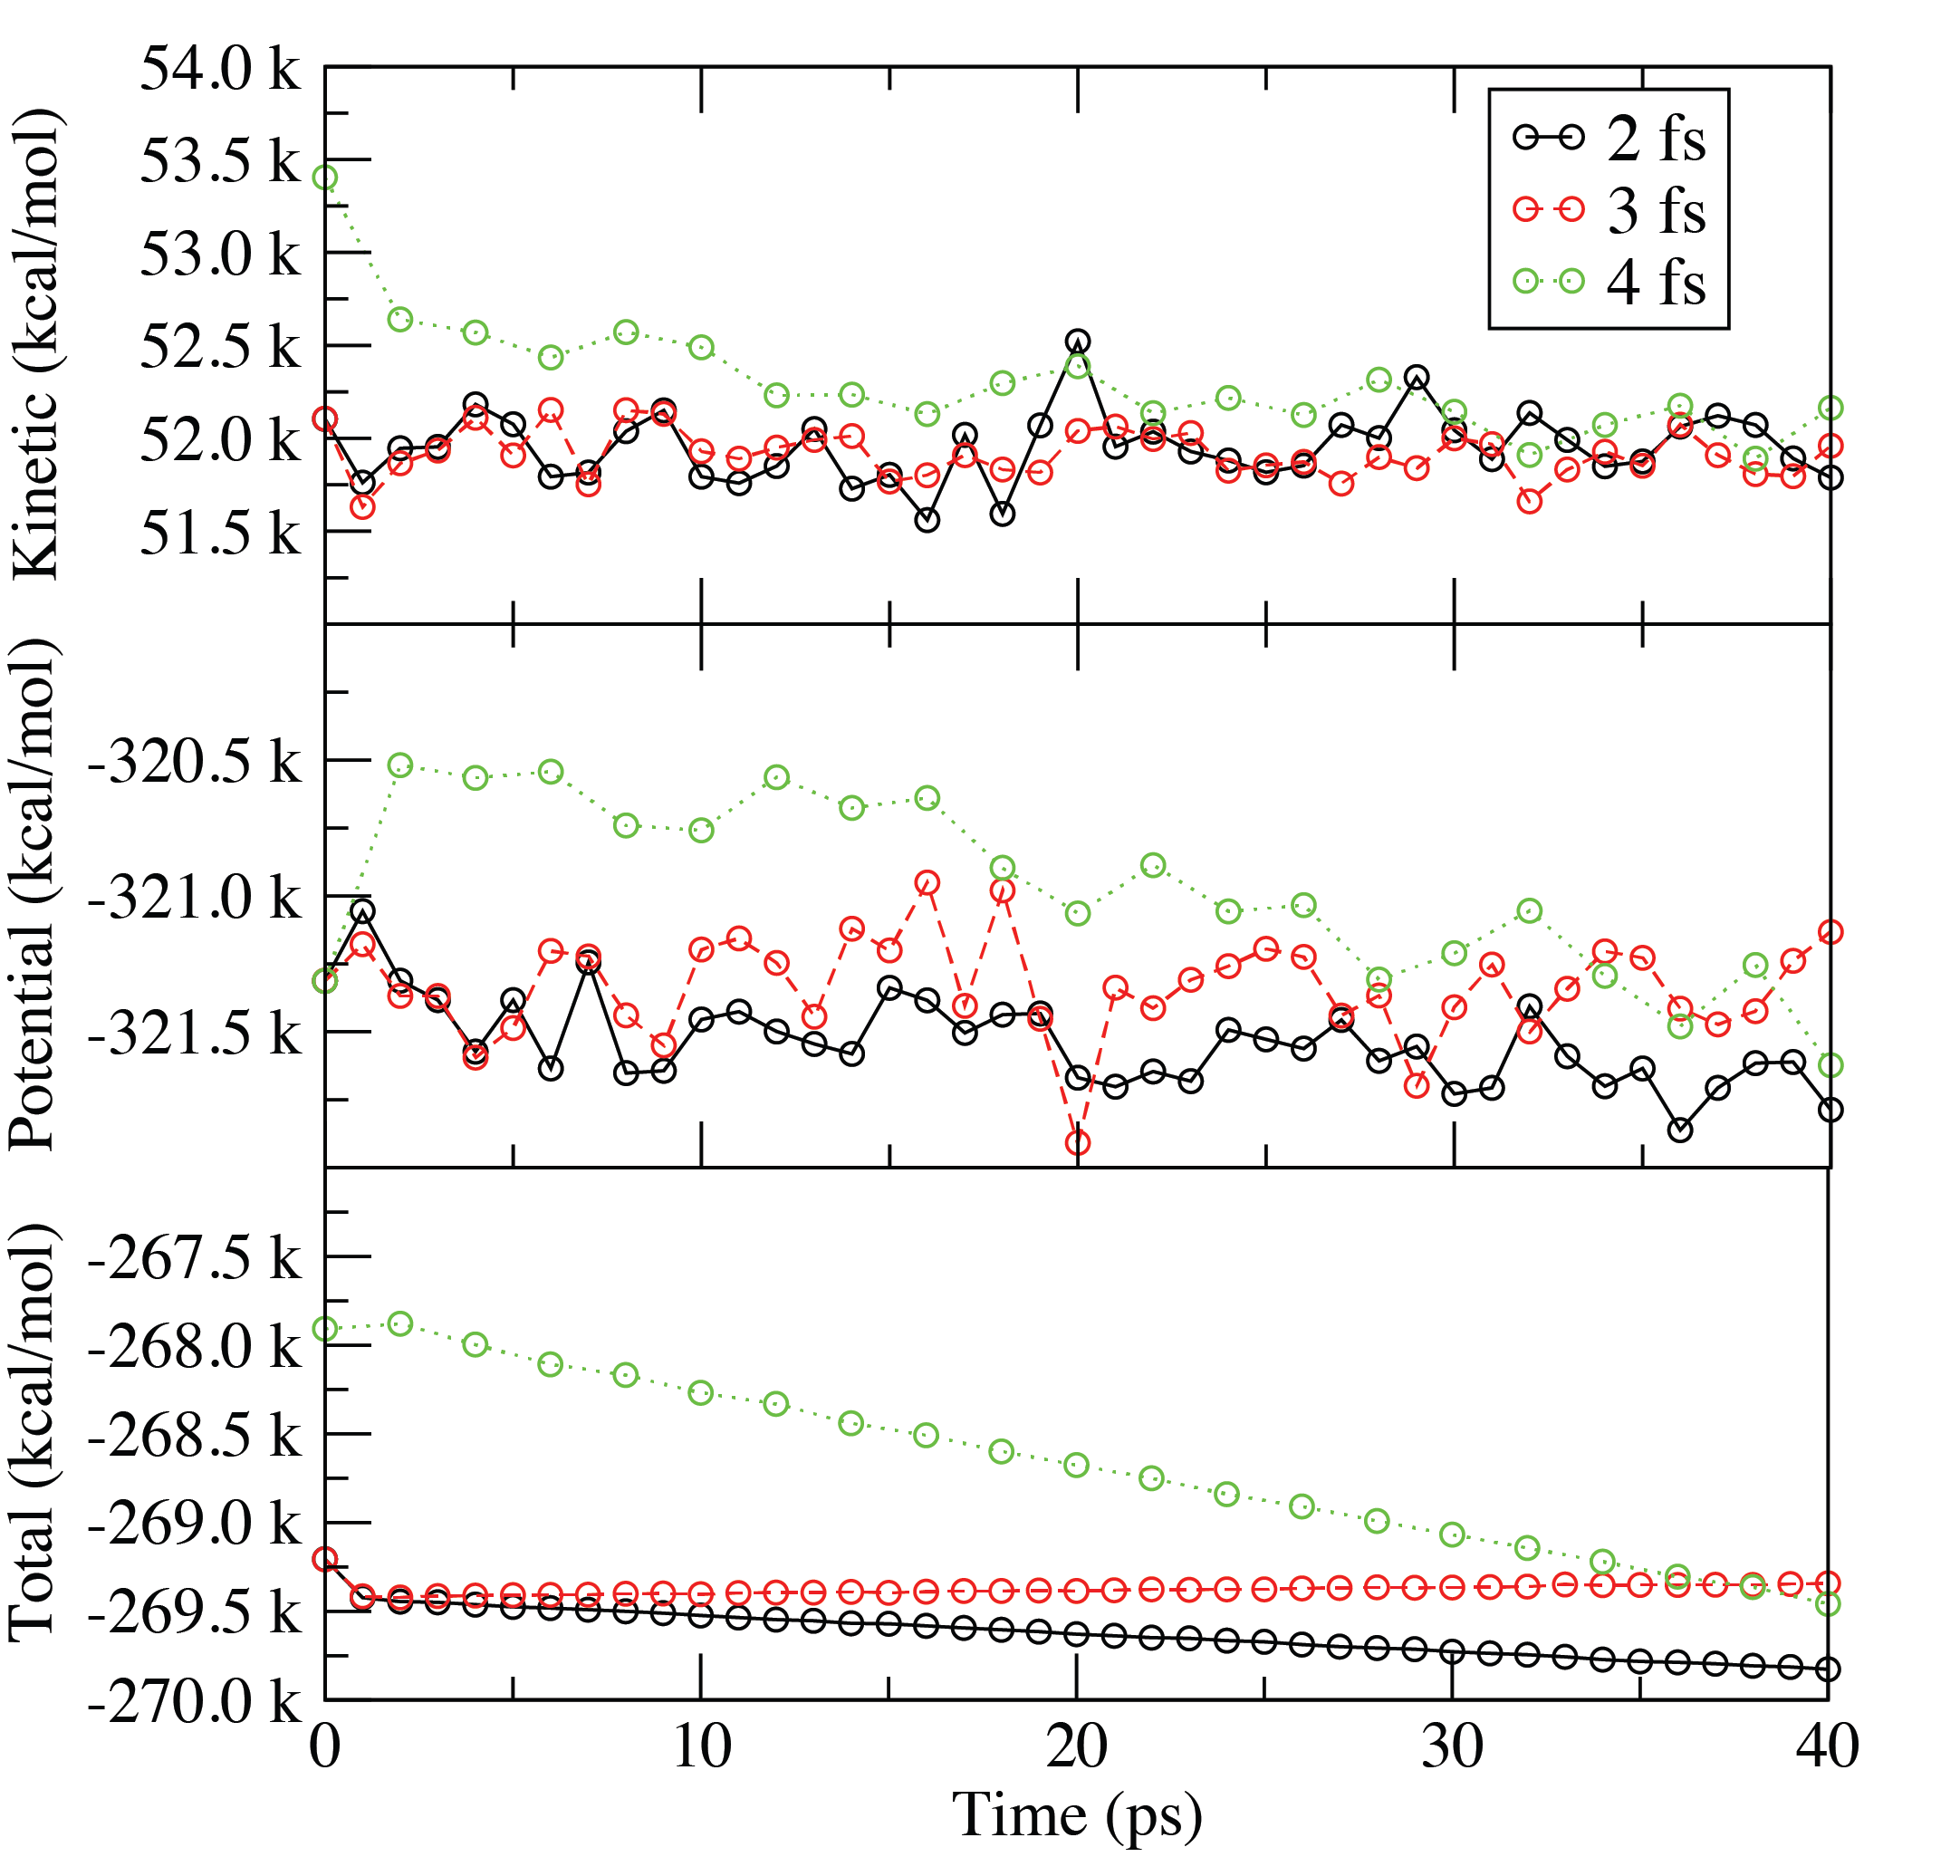
\includegraphics[scale=0.5]{ch6_fig1_timestep.png}
\caption[Energy fluctuations calculated for different integration time- steps.] {\textbf{Energy fluctuations calculated for different integration time-steps.} Simulations with constant energy (NVE) were performed to evaluate how well the total ennergy was conserved for 4 fs simulations of mPKM2$^{apo}$, using integration time steps sizes of 2 fs (black), 3 fs (red) and 4 fs (green).}
\label{fig:timestep}
\end{figure}
%
%
%%% TABLE
%
% Please add the following required packages to your document preamble:
% \usepackage{booktabs}
\begin{table}[!ht]
\begin{tabular}{@{}lll@{}}
\toprule
Time step & $\frac{\Delta E_{total}}{\Delta E_{kinetic}}$ & $\frac{\Delta E_{total}}{\Delta E_{potential}}$ \\ \midrule
2.0 & 0.2303 & 0.2317 \\
3.0 & 0.9811 & 0.8420 \\
4.0 & 1.3500 & 1.5445 \\ \bottomrule
\end{tabular}
\caption[Single precision NVE simulation without thermostat or barostat coupling.]{\textbf{Single precision NVE simulation without thermostat or barostat coupling.} Quantification of the energy fluctuations in NVE simulations of mPKM2$^{apo}$, as shown in \textbf{Fig. \ref{fig:timestep}}.}
\label{tab:timestep}
\end{table}
%
%
%
%%% TABLE
%
%
\begin{sidewaystable}
%\begin{table}[!ht]
\begin{tabular}{@{}lllll@{}}
\toprule
System            & Oligomer & Ligand                                        & Replicas & Length (ns) \\ \midrule
$mPKM2^{apo}$     & Monomer  & Apo                                           & 3        & 300         \\
$mPKM2^{FBP}$     & Monomer  & Fructose 1,6-bisphosphate                     & 5        & 300    \\
$mPKM2^{Phe}$     & Monomer  & L-phenylalanine                               & 3        & 300         \\
$mPKM2^{Tepp}$    & Monomer  & Tepp-46                                       & 3        & 300         \\
$tPKM2^{apo}$     & Tetramer & Apo                                           & 5        & 400         \\
$tPKM2^{FBP}$     & Tetramer & Fructose 1,6-bisphosphate                     & 5        & 400         \\
$tPKM2^{FBP+Ser}$ & Tetramer & Fructose 1,6-bisphosphate and L-serine        & 3        & 400         \\
$tPKM2^{FBP+Ser}$ & Tetramer & Fructose 1,6-bisphosphate and L-phenylalanine & 3        & 400         \\ \bottomrule
\end{tabular}
\caption[Summary of MD simulations of monomeric and tetrameric PKM2.]{\textbf{Summary of MD simulations of monomeric and tetrameric PKM2.} A tabular summary of explicit solvent molecular dynamics simulations performed of monomeric and tetrameric PKM2. In addition to the five replicas of 300 ns simulation of $mPKM2^{FBP}$, a single replica was continued for an additional 200 ns.}
%\end{table}
\end{sidewaystable}
\clearpage

\subsection{FBP binding causes PKM2 monomers to sample two distinct conformational states}
To investigate the mechanical response of PKM2 upon FBP and Phe binding we performed MD simulations of mPKM2$^{apo}$, mPKM2$^{FBP}$ and mPKM2$^{Phe}$ at a constant temperature of 300 K and a pressure of 1 atm. To simplify the high-dimensionality of the trajectories and to study the molecular determinants related to the binding Phe or FBP, principal component analyses were performed of the positional coordinates of the three simulations. After removing roto-translational degrees of freedom, the covariance matrix ($\sigma$) of the atomic positional fluctuations was calculated with the elements:
%
%
\begin{equation}
\sigma_{ij} = \langle (x_{i} - \langle x_i \rangle )( x_j - \langle x_j \rangle ) \rangle
\label{equ:covmat}
\end{equation}
%
%
where $\lbrace x_{1}, x_{2}, x_{3}, ..., x_{3N} \rbrace$ are the Cartesian coordinates of the protein. The covariance matrix was then trivially expressed in mass-weighted coordinates:
%
%
\begin{equation}
\sigma ' = M \sigma
\end{equation}
%
%
where $M$ is the mass matrix of the protein. From the mass-weighted covariance matrix ($\sigma '$), eigenvalues ($\lambda$) and eigenvectors ($x$) were determined through a linear transformation:
%
%
\begin{equation}
0 = (\sigma ' - I \lambda ) x
\label{equ:eigeval_prob}
\end{equation}
%
%
where $I$ is the unit matrix. The eigenvalue problem in Equ. \ref{equ:eigeval_prob} was solved for the eigenvalues and the eigenvectors of the system. 
%
%
\\\\
%
%
Simulated trajectories of mPKM2$^{FBP}$ were found to sample two discrete conformational states in eigenvector space over the course of a 500 ns simulation (\textbf{Fig. \ref{fig:monomer_pca} A}). A k-means clustering of the PCA plot found that two clusters [i] and [ii] explained all of the point variability of the data set. Transition between clusters [i] and [ii] was dominated by the movement of the B-domain into the closed conformation over the substrate-binding pocket, and a change to the N-terminal helix-loop-helix (HLH) into an alternative, stable conformation (\textbf{Fig. \ref{fig:monomer_pca} A}). The nature of the B-domain motion led to the annotation of cluster [i] as the \textit{open} conformation and cluster [ii] as the \textit{closed} conformation. 
%
%
\\\\
%
%
MD simulations of mPKM2$^{apo}$, mPKM2$^{Phe}$ and mPKM2$^{Tepp-46}$ were similarly analysed for positional variance about the first two eigenvectors by transforming their positional coordinates into eigenvector space (\textbf{Fig. \ref{fig:monomer_pca} B}). In order to project all four monomer trajectories into the same eigenvector space, the same rotation matrix was applied to each coordinate system. Analyses of mPKM2$^{apo}$ and mPKM2$^{Phe}$ trajectories were confined to cluster [i], thus sampling the \textit{open} conformation, whereas $mPKM2^{Tepp-46}$ was found to sample the closed conformation. 
%
%
%
%
%%% FIGURE
%
\begin{figure}[!ht]
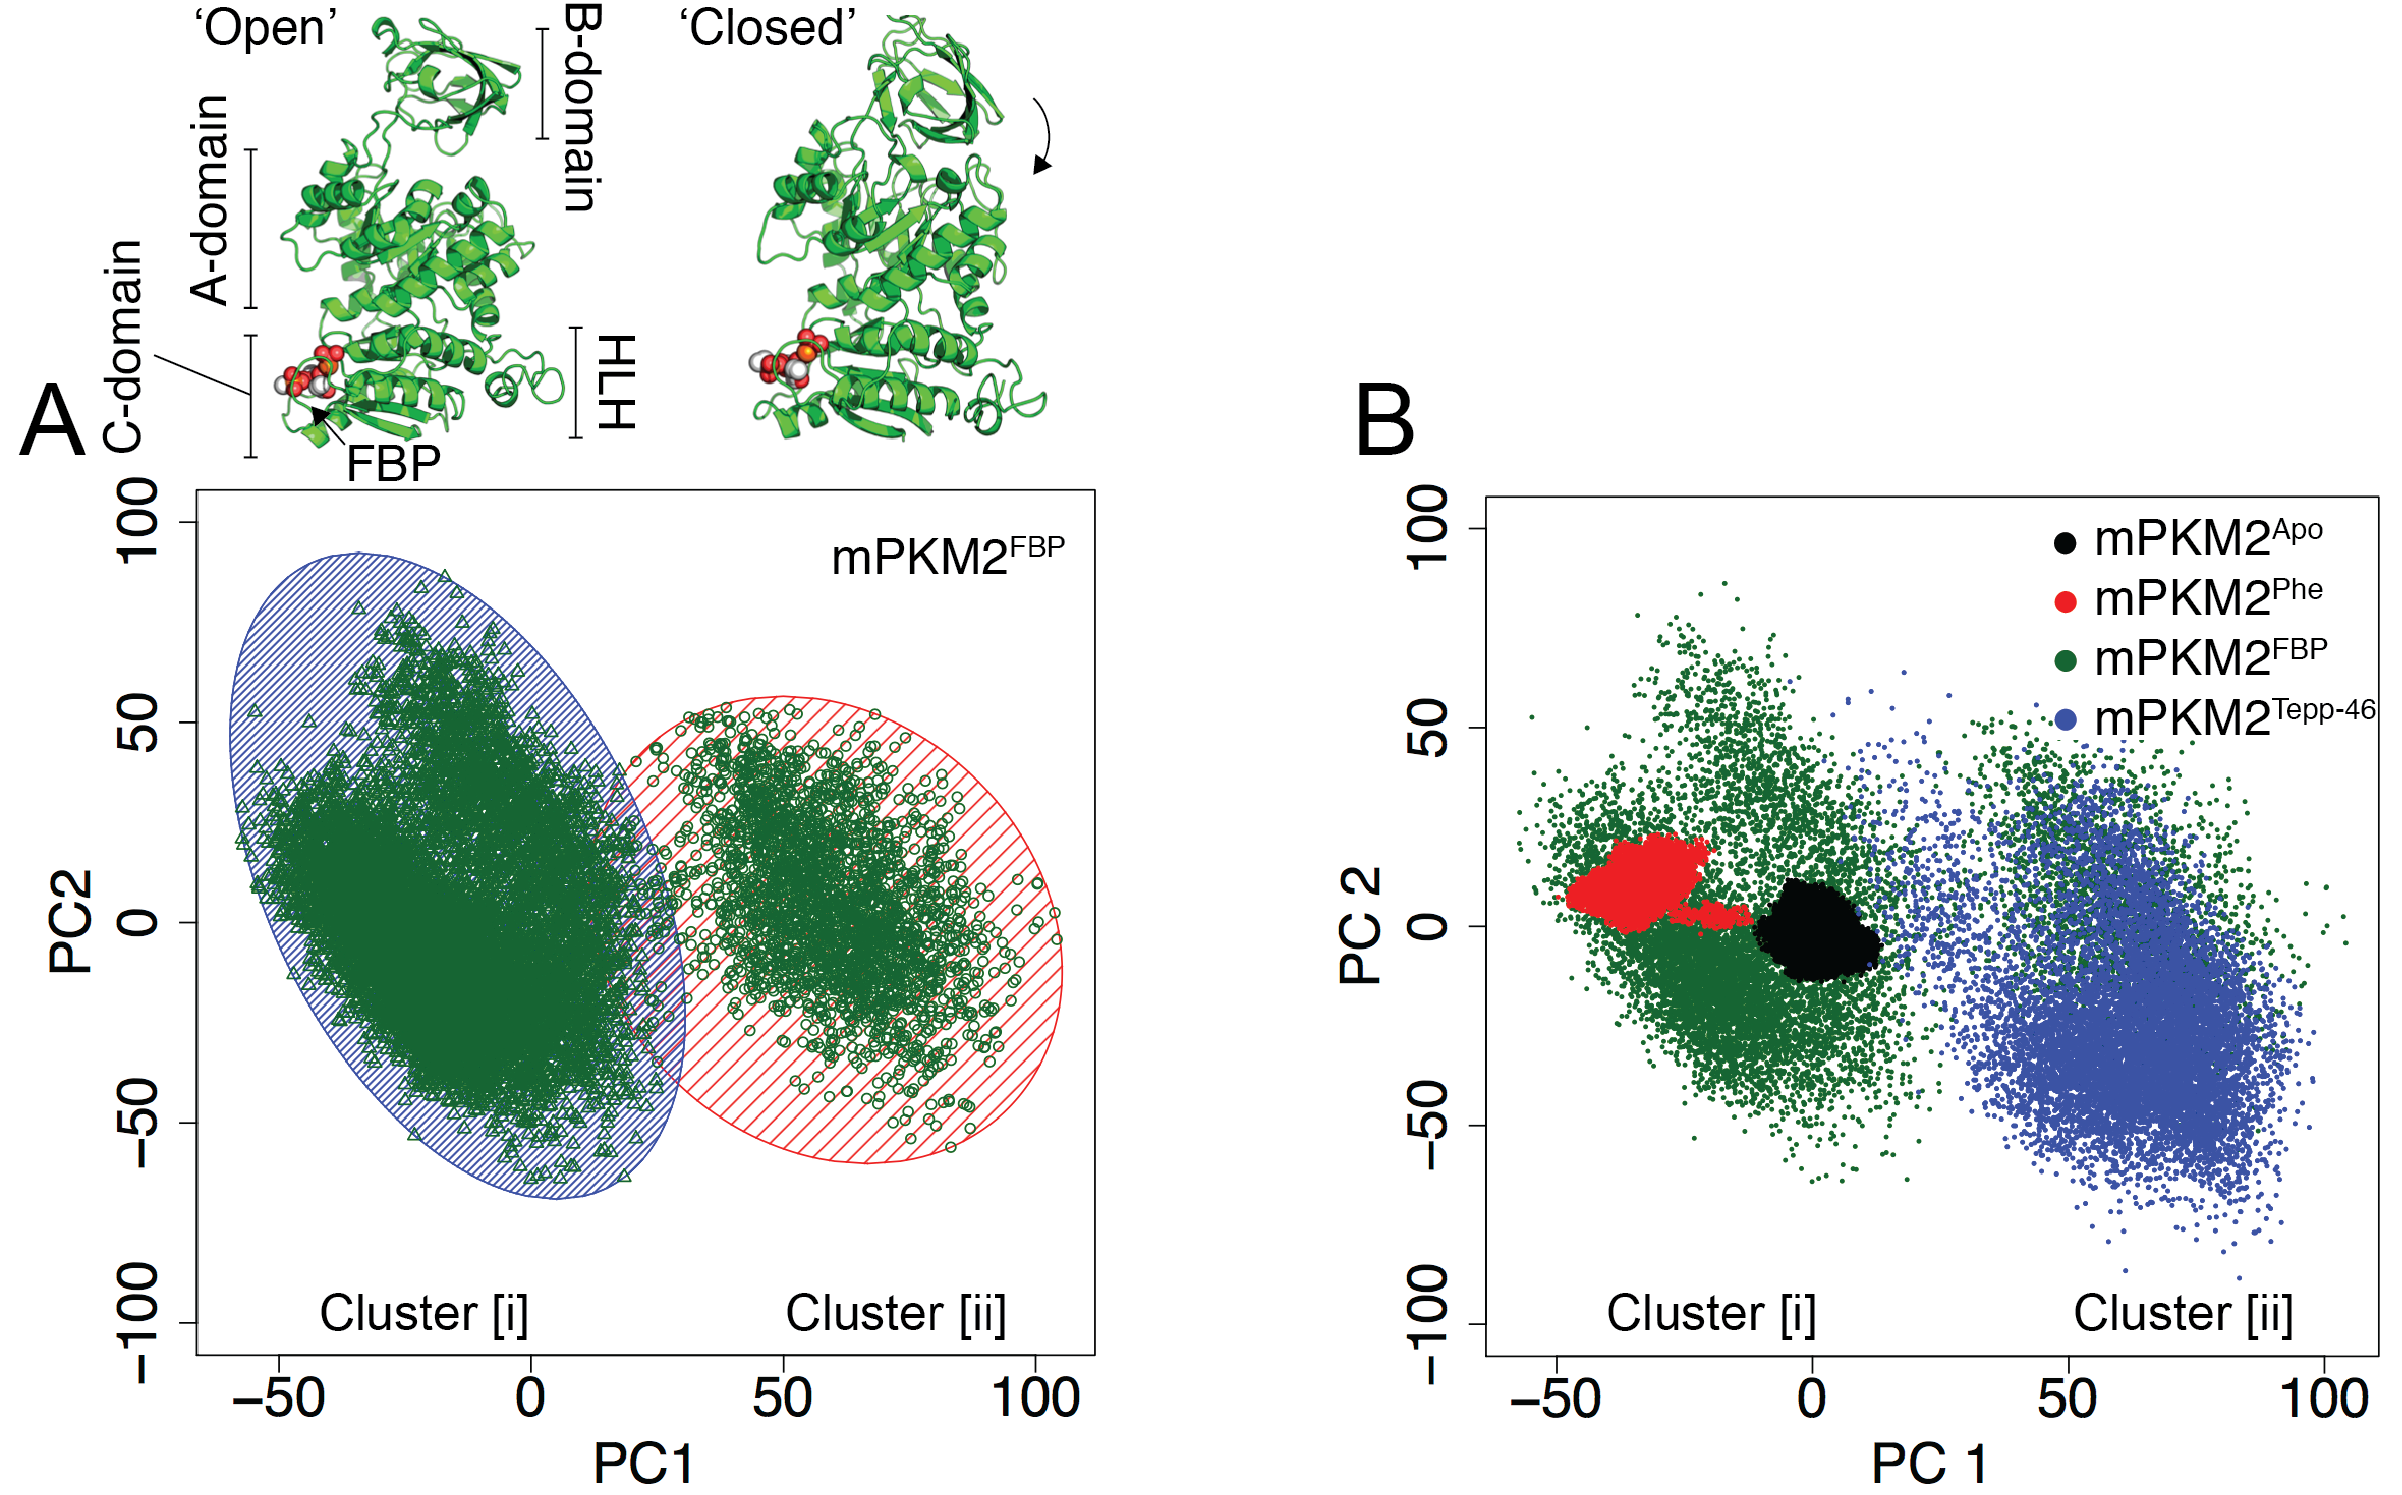
\includegraphics[scale=0.7]{ch6_fig2_monomer_pca.png}
\caption[Conformational plasticity and essential dynamics of monomeric PKM2.]{\textbf{Conformational plasticity and essential dynamics of monomeric PKM2.} \textbf{(A)} PCA projection of a 500 ns MD simulation of PKM2 bound to FBP. Two clusters were found to explain 100 \% point variability of the data set. Single most dominant conformations of $mPKM2^{FBP}$ were extract from clusters [i] and [ii] and are shown in cartoon representation above. The first eigenvector accounted for 37.5 \% of the total variance and the second eigenvector accounted for 13.1 \% of the total variance. \textbf{(B)} Superimposition of eigenvalues from $mPKM2^{apo}$ (black), $mPKM2^{Phe}$ (red) and $mPKM2^{Tepp-46}$ (blue) onto the first two eigenvectors determined from an eigenvalue decomposition of the C$\alpha$ coordinates of $mPKM2^{FBP}$ (green).}
\label{fig:monomer_pca}
\end{figure}
%
\clearpage
%
%
The \textit{open} to \textit{closed} transition of the B-domain in the first 300 ns of $mPKM2^{FBP}$ simulations was observed to occur as a single two-state transition, and a re-opening of the B-domain was not observed within this time scale. To investigate the conformational equilibrium of the B-domain state transition, MD simulations of $mPKM2^{FBP}$ were extended for a further 200 ns. The resulting B-domain cap dynamics was quantified by measuring the distance between the centre of mass of the A- and B-domains. Extended MD simulations of $mPKM2^{FBP}$  found a reversal between energy minima about the \textit{open} and \textit{closed} conformations, with an intermediate \textit{semi-closed} conformation additionally detected (\textbf{Fig. \ref{fig:monomer_b-domain} A} and \textbf{B}).
%
%
\\\\
%
%
Taken together, these data suggested that the reversible closure of the B-domain in monomeric PKM2 was dependent on FBP binding, within the simulated time scales, and that this is a feature of PKM2 activation. Consistent with this interpretation, mPKM2$^{Apo}$ and mPKM2$^{Phe}$ were found to same the open conformation, whereas $mPKM2^{Tepp}$ sampled to closed conformation (\textbf{Fig. \ref{fig:monomer_b-domain} C-E}). It was therefore hypothesised that B-domain closure contributes to enzyme activation.
%
%
%
%
%%% FIGURE
%
\begin{figure}[!ht]
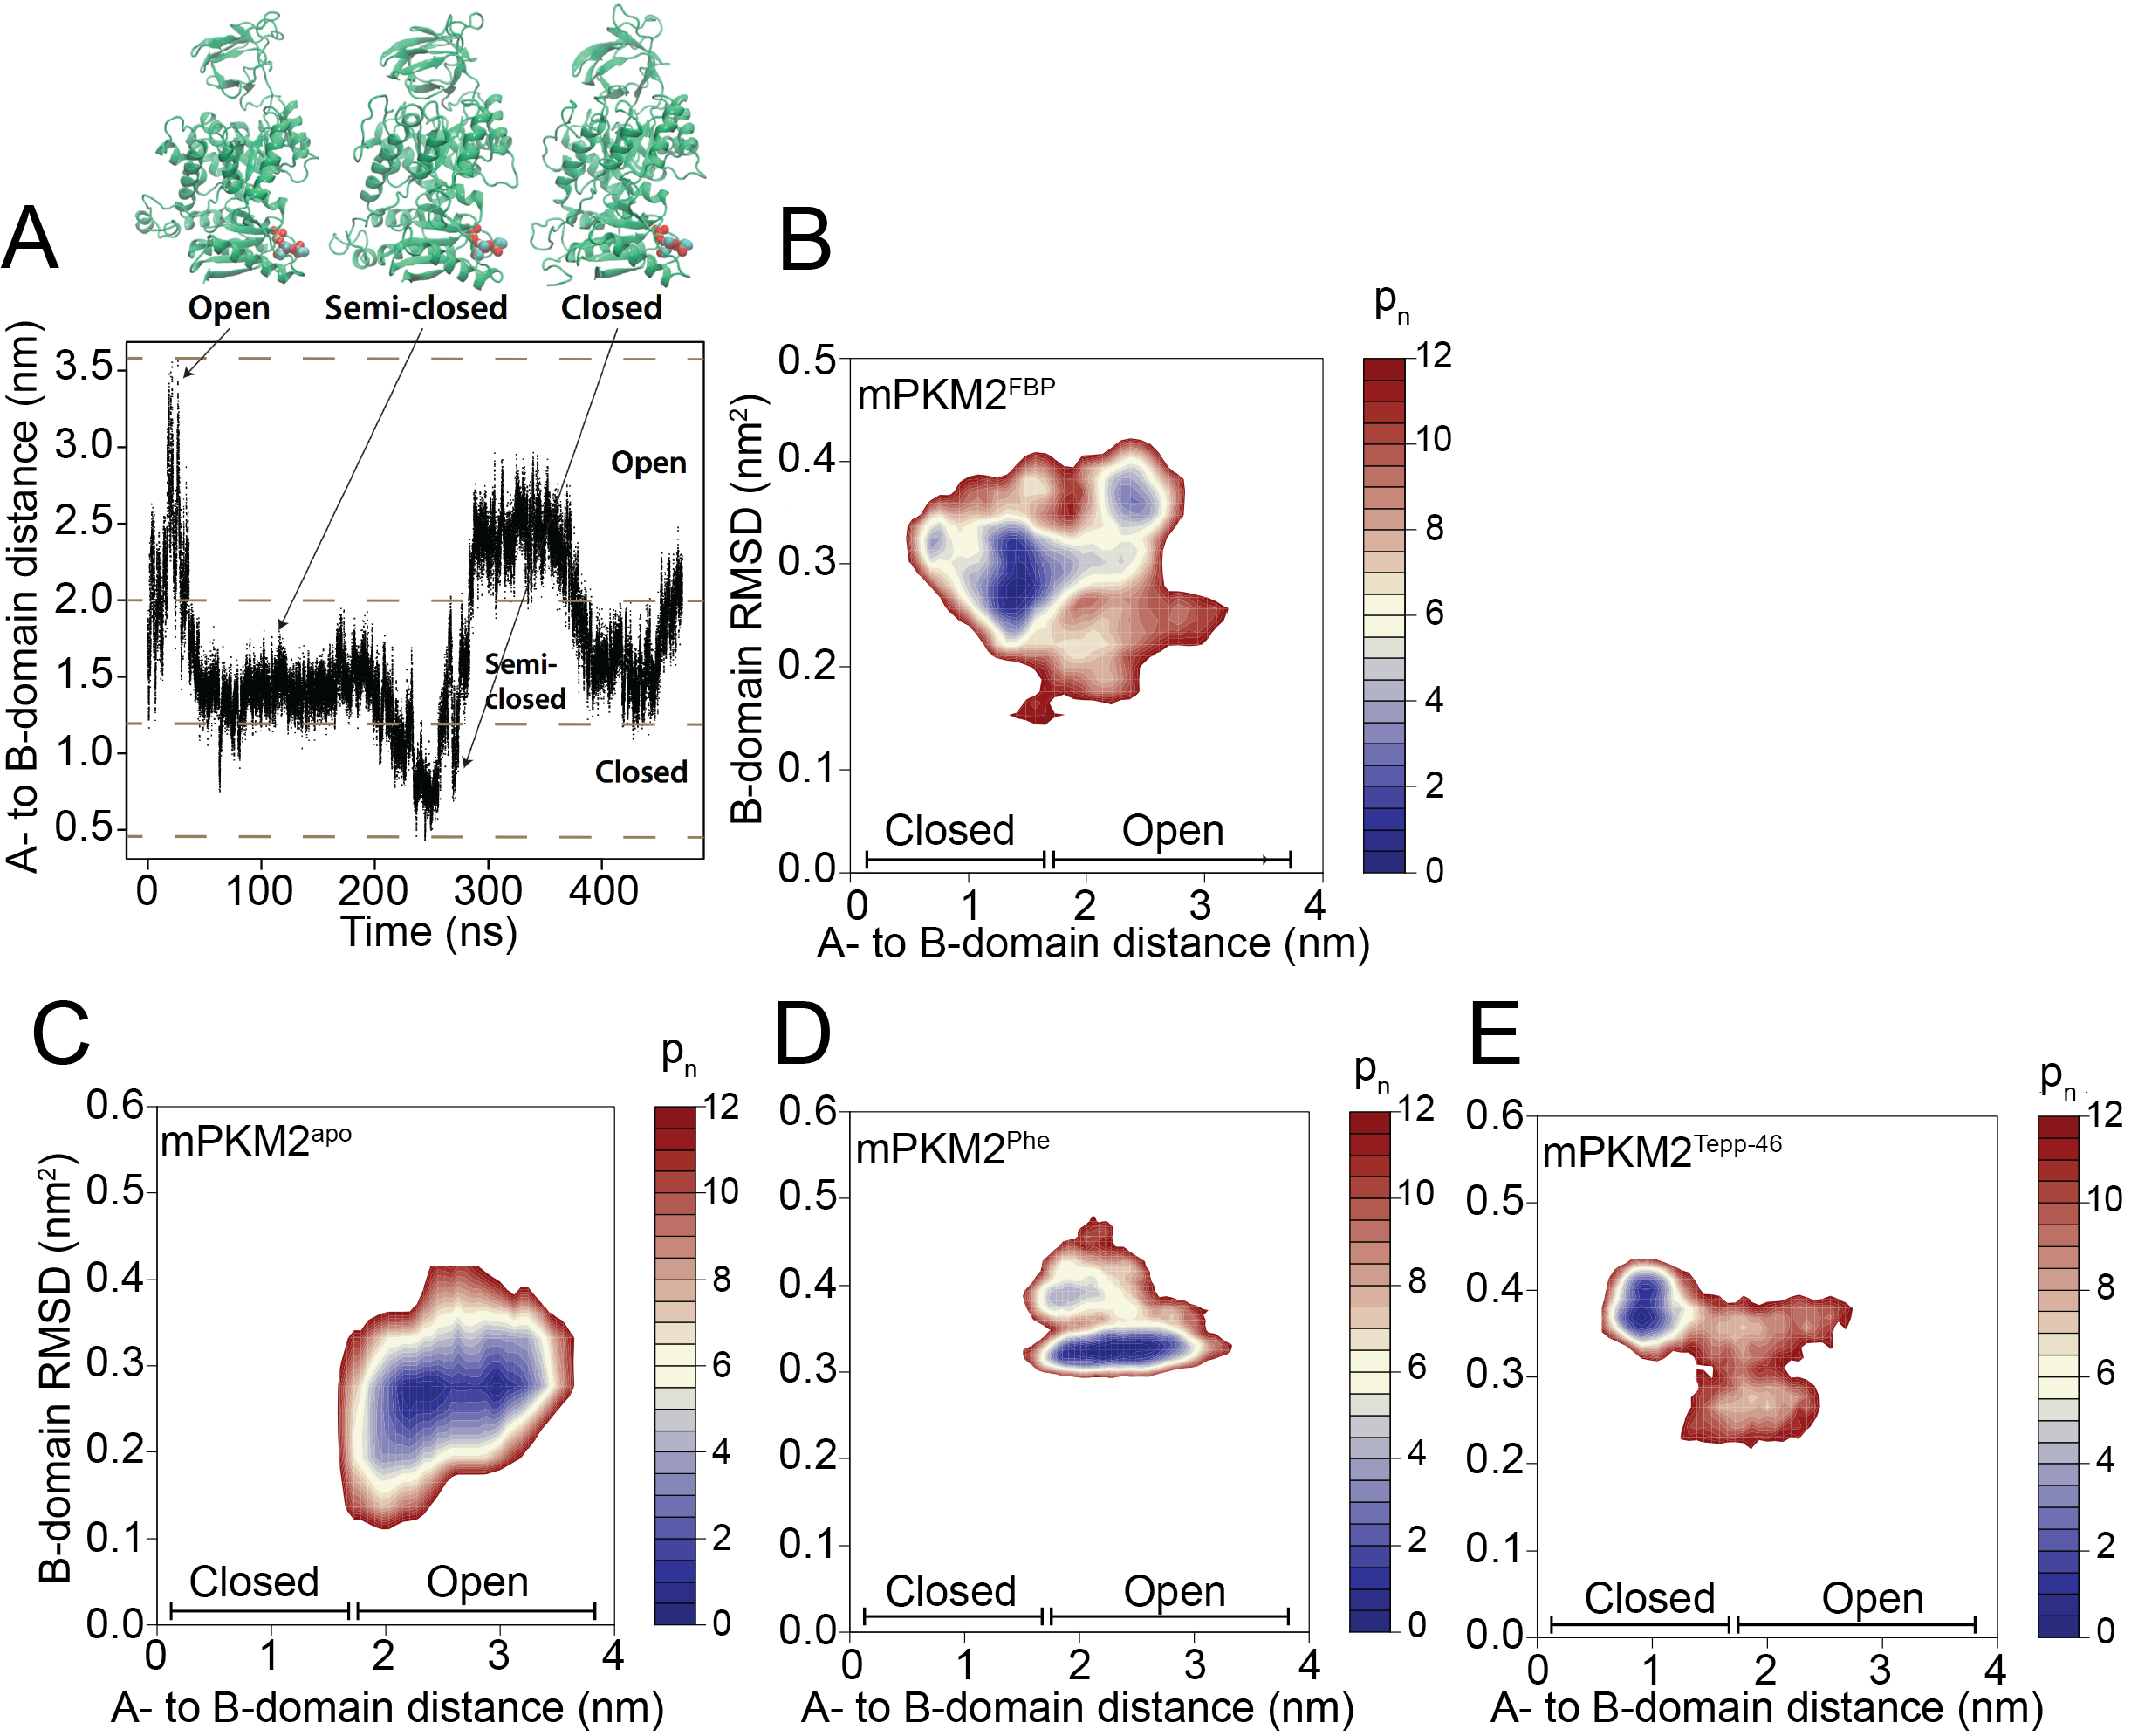
\includegraphics[scale=0.7]{ch6_fig3_bdomain.png}
\caption[Conformational equilibrium of FBP-induced cap closure from a 500 ns MD simulation.] {\textbf{Conformational equilibrium of FBP-induced cap closure from a 500 ns MD simulation.} \textbf{(A)} The distance computed between the centre of mass for the A-domain and the centre of mass of the B-domain over the course of an MD simulation of $mPKM2^{FBP}$. Surface distribution of states plot, with Boltzmann averages of states calculated by B-domain cap distance as a function of the RMSD of the B-domain for \textbf{(B)} $mPKM2^{FBP}$, \textbf{(C)} $mPKM2^{Apo}$, \textbf{(D)} $mPKM2^{Phe}$ and \textbf{(E)} $mPKM2^{Tepp}$.}
\label{fig:monomer_b-domain}
\end{figure}

\clearpage


\subsection{B-domain closure traps highly resident water molecules in the active site}
previous studies have found that a water molecule is required as part of the catalytic mechanism of PKM2 to protonate the enolate intermediate \cite{Hollenberg:1971aa}. This is supported by crystal structures of PKM2 showing a cluster of water molecules proximal to the active site residues T328 and S362 \cite{Christofk:2008aa,Dombrauckas:2005aa}. In light of the observation of ligand-dependent B-domain dynamics affecting the solvent exposure of the catalytic pocket, we postulated that the closure of the B-domain would affect the solvent dynamics in the catalytic pocket and that this may play a role in catalysis. 
%
%
\\\\
%
%
An analysis of water density maps \cite{Fornili:2012aa} calculated from representative structures from MD simulations of $mPKM2^{FBP}$ in the \textit{open} and the \textit{closed} conformations, found that the active site pocket contained an increased number of highly resident water molecules when the B-domain cap was closed (\textbf{Fig. \ref{fig:monomer_water_residence}}). Moreover, a cluster of resident water molecules were positioned proximal to T382 and S362 in the closed state. This would suggest that B-domain closure contributes to catalysis by trapping necessary water molecules, proximal to the substrate binding pocket. 
%
%
%
%
%%% FIGURE
%
\begin{figure}[!ht]
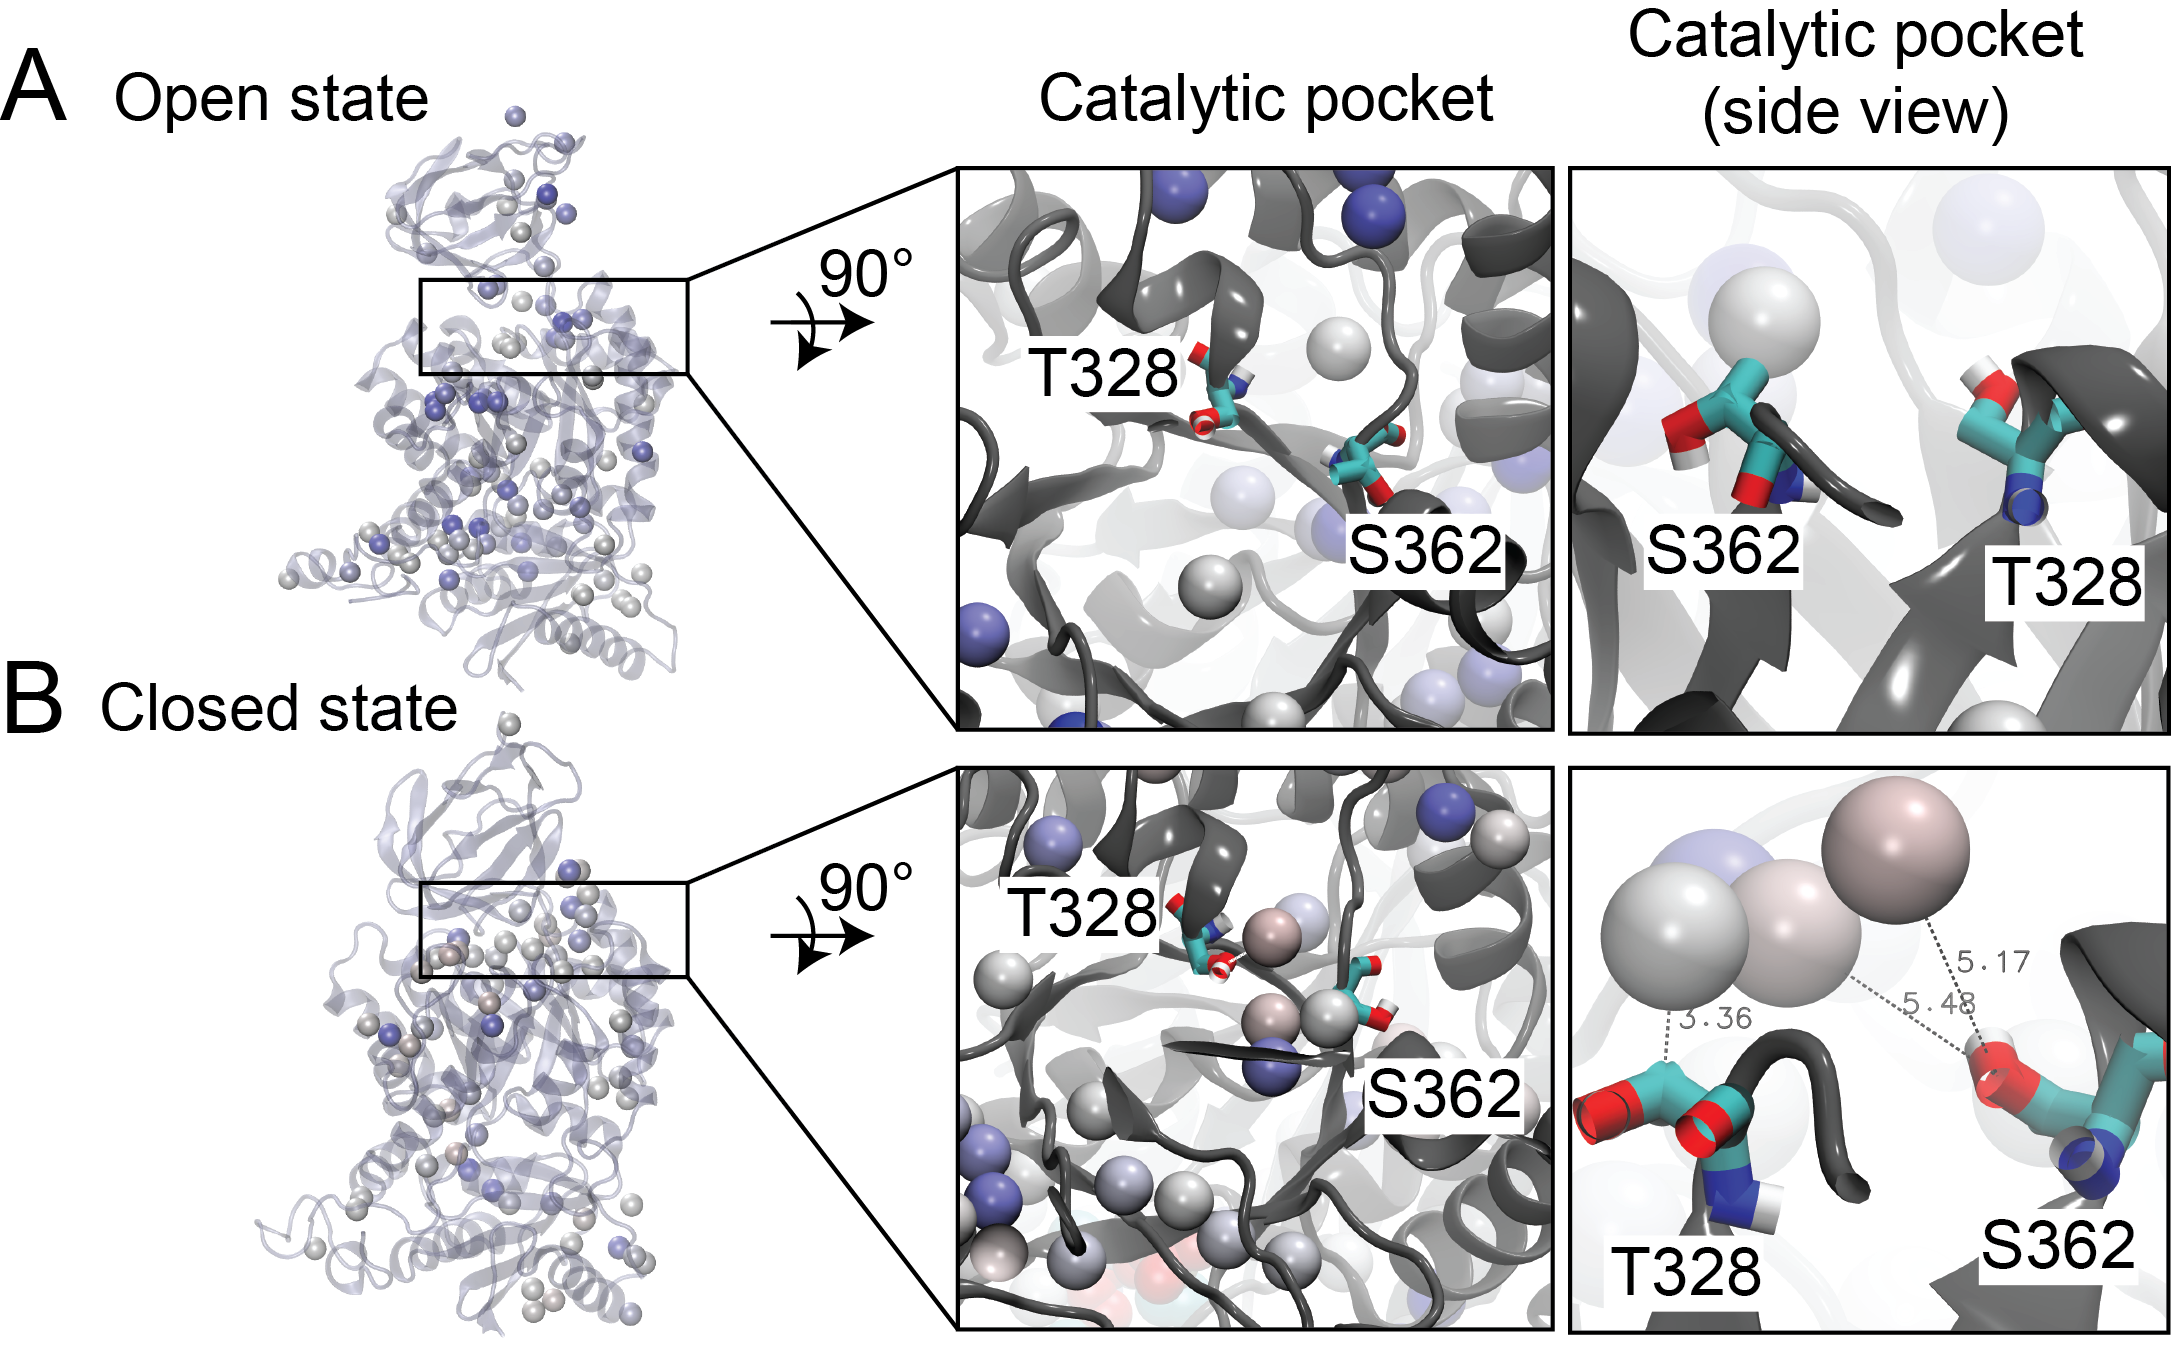
\includegraphics[scale=0.6]{ch6_fig5_active_site_water.png}
\caption[Water residence time at the active site of mPKM2-FBP.]{\textbf{Water residence time at the active site of mPKM2-FBP.} Water density was calculated on a 0.5 \AA -spaced grid and averaged over snapshots exracted from the mPKM2-FBP simulation every 0.1 ps for the \textbf{(A)} open and \textbf{(B)} closed conformations of the B-domain cap. The hydration sites (spheres) are coloured from white to blue according to increased water density.}
\label{fig:monomer_water_residence}
\end{figure}

\clearpage


\subsection{B-domain dynamics is correlated with structural changes to catalytic residues in the active site}
%
%
To further explore whether B-domain closure was accompanied by other features of PKM2 activation, we investigated the side-chain dynamics at the active site of the protein. A superimposition of PKM2 active site residues from crystal structures deposited in the protein data-bank, found that the catalytic residue H78 adopts an altered side-chain conformation when the protein is bound to allosteric activators FBP and Tepp-46 (PDB ID: 3u2z) and L-serine and FBP (PDB ID: 4b2d), compared to crystal structures of apo PKM2 (PDB ID: 3bjt) and PKM2 bound to the inhibitor phenylalanine (PDB ID: 4fxj) (\textbf{Fig. \ref{fig:monomer_h78_chi2} A}). H78 has been implicated the phospho-transfer reaction of PKM2 as a proton-donor and acceptor in the catalytic cycle \cite{Hollenberg:1971aa}.  In the activator-bound structures, the $N_{\delta 1}$ group was found to be positioned towards the active site, and was found positioned away from the active site in apo- and Phe-bound structures (\textbf{Fig. \ref{fig:monomer_h78_chi2} A}). Consistent with this change following allosteric activator binding, the conformation of H78 was proposed to provide a potential read-out for whether PKM2 was in the active or the inactive states. 
%
%
\\\\
%
%
To investigate possible changes to the orientation of H78 in the MD simulations of PKM2, the $\chi_{2}$ torsion angle of H78 was measured in simulations of mPKM2$^{FBP}$ and mPKM2$^{apo}$. We found that the closure of the B-domain was accompanied by the catalytic H78 adopting a $\chi_{2}$ torsion angle of between \ang{100} and \ang{110}, in agreement with the $\chi_{2}$ torsion angles of the crystal structures of activator-bound PKM2 (\ang{108.2} for PKM2$^{FBP + Ser}$ and \ang{103.0} for PKM2$^{FBP + Tepp}$; \textbf{Fig. \ref{fig:monomer_h78_chi2} A}). Conversely simulations of mPKM2$^{apo}$ and mPKM2$^{Phe}$ displayed variable H78 $\chi_{2}$ torsion angles approximately equivalent to that the inhibited crystal structures ($\simeq$ \ang{-70}; \textbf{Fig. \ref{fig:monomer_h78_chi2} A}). This further suggested that the \textit{open} conformation corresponds to the inactive state of PKM2 and that FBP-induced closure of the B-domain contributed to the transition to the active state.
%
%
%
%
%%% FIGURE
%
\begin{figure}[!ht]
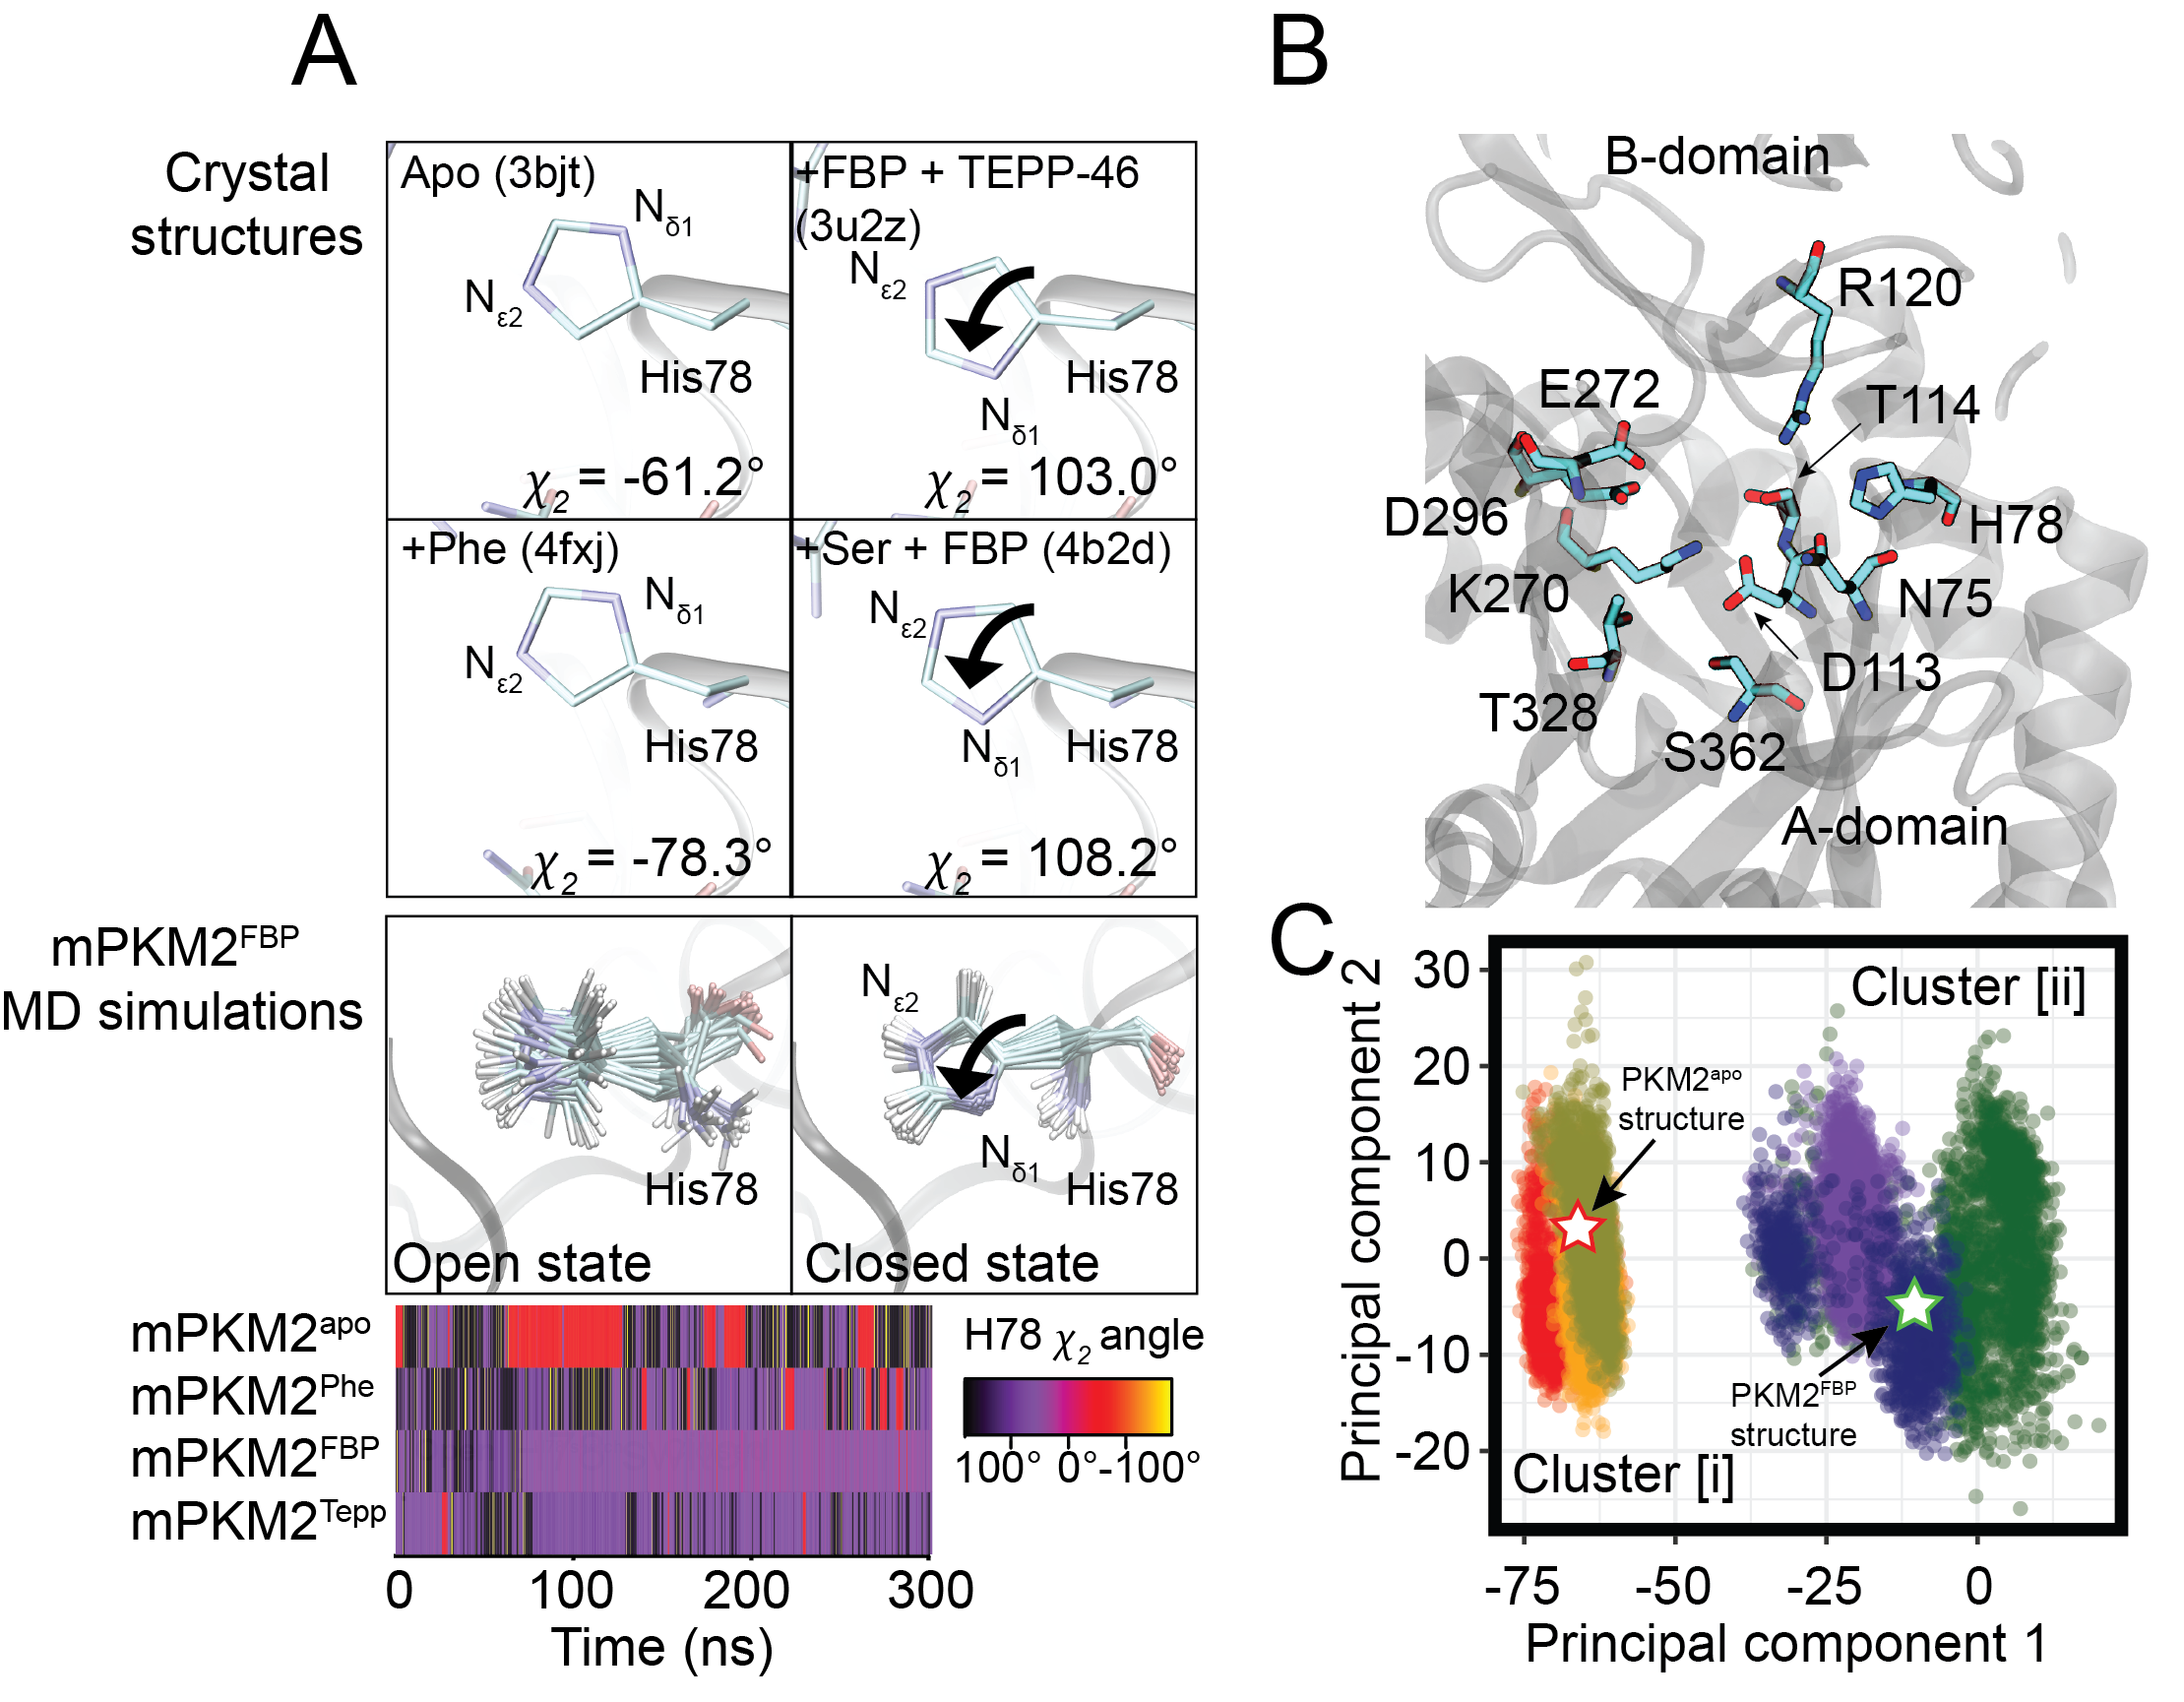
\includegraphics[scale=0.76]{ch6_fig4_h78_chi2.png}
\caption[Active site residue H78 adopts a distinct side-chain conformation depending on the liganded state of the protein.] {\textbf{Active site residue H78 adopts a distinct side-chain conformation depending on the liganded state of the protein.} \textbf{(A)} The active site residue histidine 78 (H78) shown in stick representation for crystal structures of apo- FBP and activator-, phenylalanine-, and serine and FBP-bound PKM2. Below, 18 evenly spaced snap-shots of the conformation of H78 are shown for a MD simulated trajectory of $mPKM2^{FBP}$ in the open and following the transition to the closed states. In the open state [Cluster (i) in Fig. \ref{fig:monomer_pca} A], the side chain of H78 is flexible and switches into a conformation seen in that of the active crystal structures following the transition of the simulation into cluster ii [Cluster (ii) in Fig. \ref{fig:monomer_pca} B]. The time evolution of the dihedral angle of H78 along MD simulations of $mPKM2^{apo}$, $mPKM2^{Phe}$, $mPKM2^{FBP}$ and $mPKM2^{Tepp-46}$, colour-coded according to the scale on the right. \textbf{(B)} The PKM2 catalytic pocket, annotated to show the active site residues. \textbf{(C)} C$\alpha$ active site corrdinates of the $mPKM2^{apo}$ active site (gold), $mPKM2^{Phe}$ (red), $tPKM2^{apo}$ (orange), $mPKM2^{FBP}$ (green), $mPKM2^{Tepp-46}$ (blue) and $tPKM2^{FBP}$ (purple) are projected onto the first two eigenvectors of $mPKM2^{FBP}$. This figure is partially adapted from \cite{Gehrig:2017aa}, which is made available under a Creative Commons Attribution license (CC-BY).}
\label{fig:monomer_h78_chi2}
\end{figure}
%
\clearpage
%
%
%
While the orientation of H78 correlated with the activity status of the crystal structures, we could not exclude the possibility that the observed flipping of the imidazole side chain of H78 was an artefact of the structure-refinement process. Therefore, a PCA analysis of the positional coordinates was performed for all active site residues (\textbf{Fig. \ref{fig:monomer_h78_chi2} B}) in simulations of mPKM2$^{apo}$, mPKM2$^{Phe}$, mPKM2$^{Tepp}$, mPKM2$^{FBP}$, tPKM2$^{apo}$ and tPKM2$^{FBP}$. This analysis found that the simulations could be separated into two clusters. The first cluster [i] contained coordinates of mPKM2$^{apo}$, mPKM2$^{Phe}$ and tPKM2$^{apo}$, while the second cluster [ii] contained coordinates of mPKM2$^{FBP}$, mPKM2$^{Tepp}$ and tPKM2$^{FBP}$ (\textbf{Fig. \ref{fig:monomer_h78_chi2} C}). Moreover, crystal structures of PKM2$^{apo}$ (PDB ID: 3bjt) and PKM2$^{FBP}$ (PDB ID: 3u2z) localized to the first and second clusters, respectively. Together, this suggested that side-chain active site changes were involved in the inactive-active transition. Nevertheless, the partition of \textit{active} and \textit{inactive} simulations into the two clusters observed in the PCA analysis of active site residues persisted for the entirety of the simulations and transitions between clusters [i] and [ii] is not observed for simulated trajectories of mPKM2$^{FBP}$. This suggested that an active-to-inactive transition, upon B-domain closure, does not completely describe the mechanism of enzyme activation. 

\clearpage


\subsection{Comparative dynamics between tetrameric and monomeric PKM2}
\label{subsec:tet_bdomain_closure}
Investigation of the oligomeric state of PKM2 by native mass spectrometry in Chapter 4 found that FBP binding results in tetramerisation. Moreover, additional experiments found that Phe and Ser compete for binding to modulate PKM2 activity, in the context of constitutive FBP binding.  
%
%
\\\\
%
%
\textcolor{red}{There are two distinct dimer interfaces within the PKM2 tetramer; the A-A' interface between the A- and C-domains of chains 1 and 2 and chains 3 and 4, and the C-C' domains between the C-domains of chains 1 and 3, and chains 2 and 4. The C-C' domain of PKM2 is formed of adjacent C-domains aligning in a 'tail-to-tail' fashion and interacts in a four-helical bundle. Particularly prominent to the C-C' domain interface is the protrusion of Lys-421 across the interface and through the loop between residues 399 to 407 on the adjacent monomer. This loop into which Lys-421 extends has a negative electrostatic potential and thus forms the basis for several charged interactions with Glu-409 and Try-443. In contrast, the A-A' interface largely encompasses several contacts between adjacent A-domains of chains 1 and 3 and chains 2 and 4, with additional bonds formed between the B-domains and N-terminal helix-loo-helix domains of the adjacent chains. Notably, helix 11 (residues 341-353) protrude into a lipophilic pocket within the first 34 residues of the N-terminal helix-loop-helix domain and the top half of helix 12 (residues 368-378) of the opposing monomer. The apparent dissociation constant of PKM2 hetero-oligomerisation measured using MST in Chatper 3 (see \textbf{Table \ref{tab:oligo_kds}}) was found to be 0.9 $\mu$M and the concentration of PKM2 in three cultured cell lines was approximately 2 $\mu$M. Given that the apparent dissociation constant of PKM2 oligomerisation is similar to its cellular concentration, PKM2 may undergo reversible oligomerisation in a cellular context. The monomer-dimer-tetramer equilibrium subsequently described in Chapter 4 is likely perturbed in cells by ligands and other interacting partners. Nevertheless, a robust description of the the cellular nature of the oligomeric equilibrium of PKM2 would necessitate further \textit{in situ} experimentation. To provide a more detailed physico-chemical model of PKM2 dynamics, tetrameric PKM2 was simulated in the apo-form (tPKM2$^{apo}$), bound to FBP (tPKM2$^{FBP}$), bound to FBP and Phe (tPKM2$^{FBP+Phe}$) and bound to FBP and Ser (tPKM2$^{FBP+Ser}$).} 
%
%
\\\\
%
%
In contrast to MD simulations of monomeric PKM2, analyses of tetrameric PKM2 MD trajectories did not show the same FBP-dependent lateral B-domain closure over the active site, as for mPKM2$^{FBP}$. Rather, an inspection of the simulated trajectories of tPKM2$^{FBP}$ found that a network of inter-protomeric charge-charge interactions was established between R342 and two aspartate residues (D178 and D179) on a flexible loop of the B-domain on the adjacent protomer. This charged interaction was observed to form after approximately 10 ns of the simulation resulting in a \textit{twisting} of the B-domain cap (\textbf{Fig. \ref{fig:tet_bdomain} A}). The positioning of the R342 side-chain was such that it blocked the B-domain cap from closing laterally over the active site, by flipping into the far side of the active site pocket (\textbf{Fig. \ref{fig:tet_bdomain} B}). In contrast, while the position of R342 and the other residues at the A-A' interface is largely similar between the crystal structures of tPKM2$^{apo}$ and tPKM2$^{FBP}$ (\textbf{Fig. \ref{fig:tet_bdomain} A}), an inspection of simulated trajectories of tPKM2$^{apo}$ found that R342 flipped away from the neighbouring active site pocket and the B-domain of the opposite protomer (\textbf{Fig. \ref{fig:tet_bdomain} B}). 
%
%
\\\\
%
%
The distance between R342 and D179 was quantified from MD trajectories of tPKM2$^{apo}$, tPKM2$^{FBP}$, tPKM2$^{FBP+Ser}$ and tPKM2$^{FBP+Phe}$ (\textbf{Fig. \ref{fig:tet_bdomain} C}). The formation of charged interactions about the interface of tPKM2$^{FBP}$ was reflected in the short inter-atomic distance between the R342 guanidino group and the acidic side-chain of D177, whereas MD trajectories of tPKM2$^{apo}$ showed distances out of the range for charged-charged interactions between these two residues (\textbf{Fig. \ref{fig:tet_bdomain} C [i] and [ii]}). A similar molecular behaviour to $tPKM2^{FBP}$ was observed in simulated trajectories of tPKM2$^{FBP+Ser}$ in the proximity between R342 and D177, resulting from a lateral twisting of the B-domain cap (\textbf{Fig. \ref{fig:tet_bdomain} C [iii]}). Conversely, the A-A' interface of tPKM2$^{FBP+Phe}$ was less compact, owing to a greater distance between R342 and D177, in a manner similar to the dynamics of tPKM2$^{apo}$ (\textbf{Fig. \ref{fig:tet_bdomain} C [iv]}).
%
%
\\\\
%
%
Taken together, an analysis of MD simulations of tetrameric PKM2 found that the conformational dynamics of the B-domain is different to that of the monomer due to steric hindrance of lateral B-domain movement by interface residues. Nevertheless, charged interactions between R342 and D177 at the A-A' interface appeared when the tetramer was bound to allosteric activators FBP and concurrently to FBP and Ser, resulting in twisting of the B-domain and an observed structural tightening. Conversely, the apo- and FBP and Phe-bound tetramers did not show this behaviour, suggesting that ligand-dependent conformational changes may accompany PKM2 regulation. 
%
%
%
%
%%% FIGURE
%
\begin{figure}[!ht]
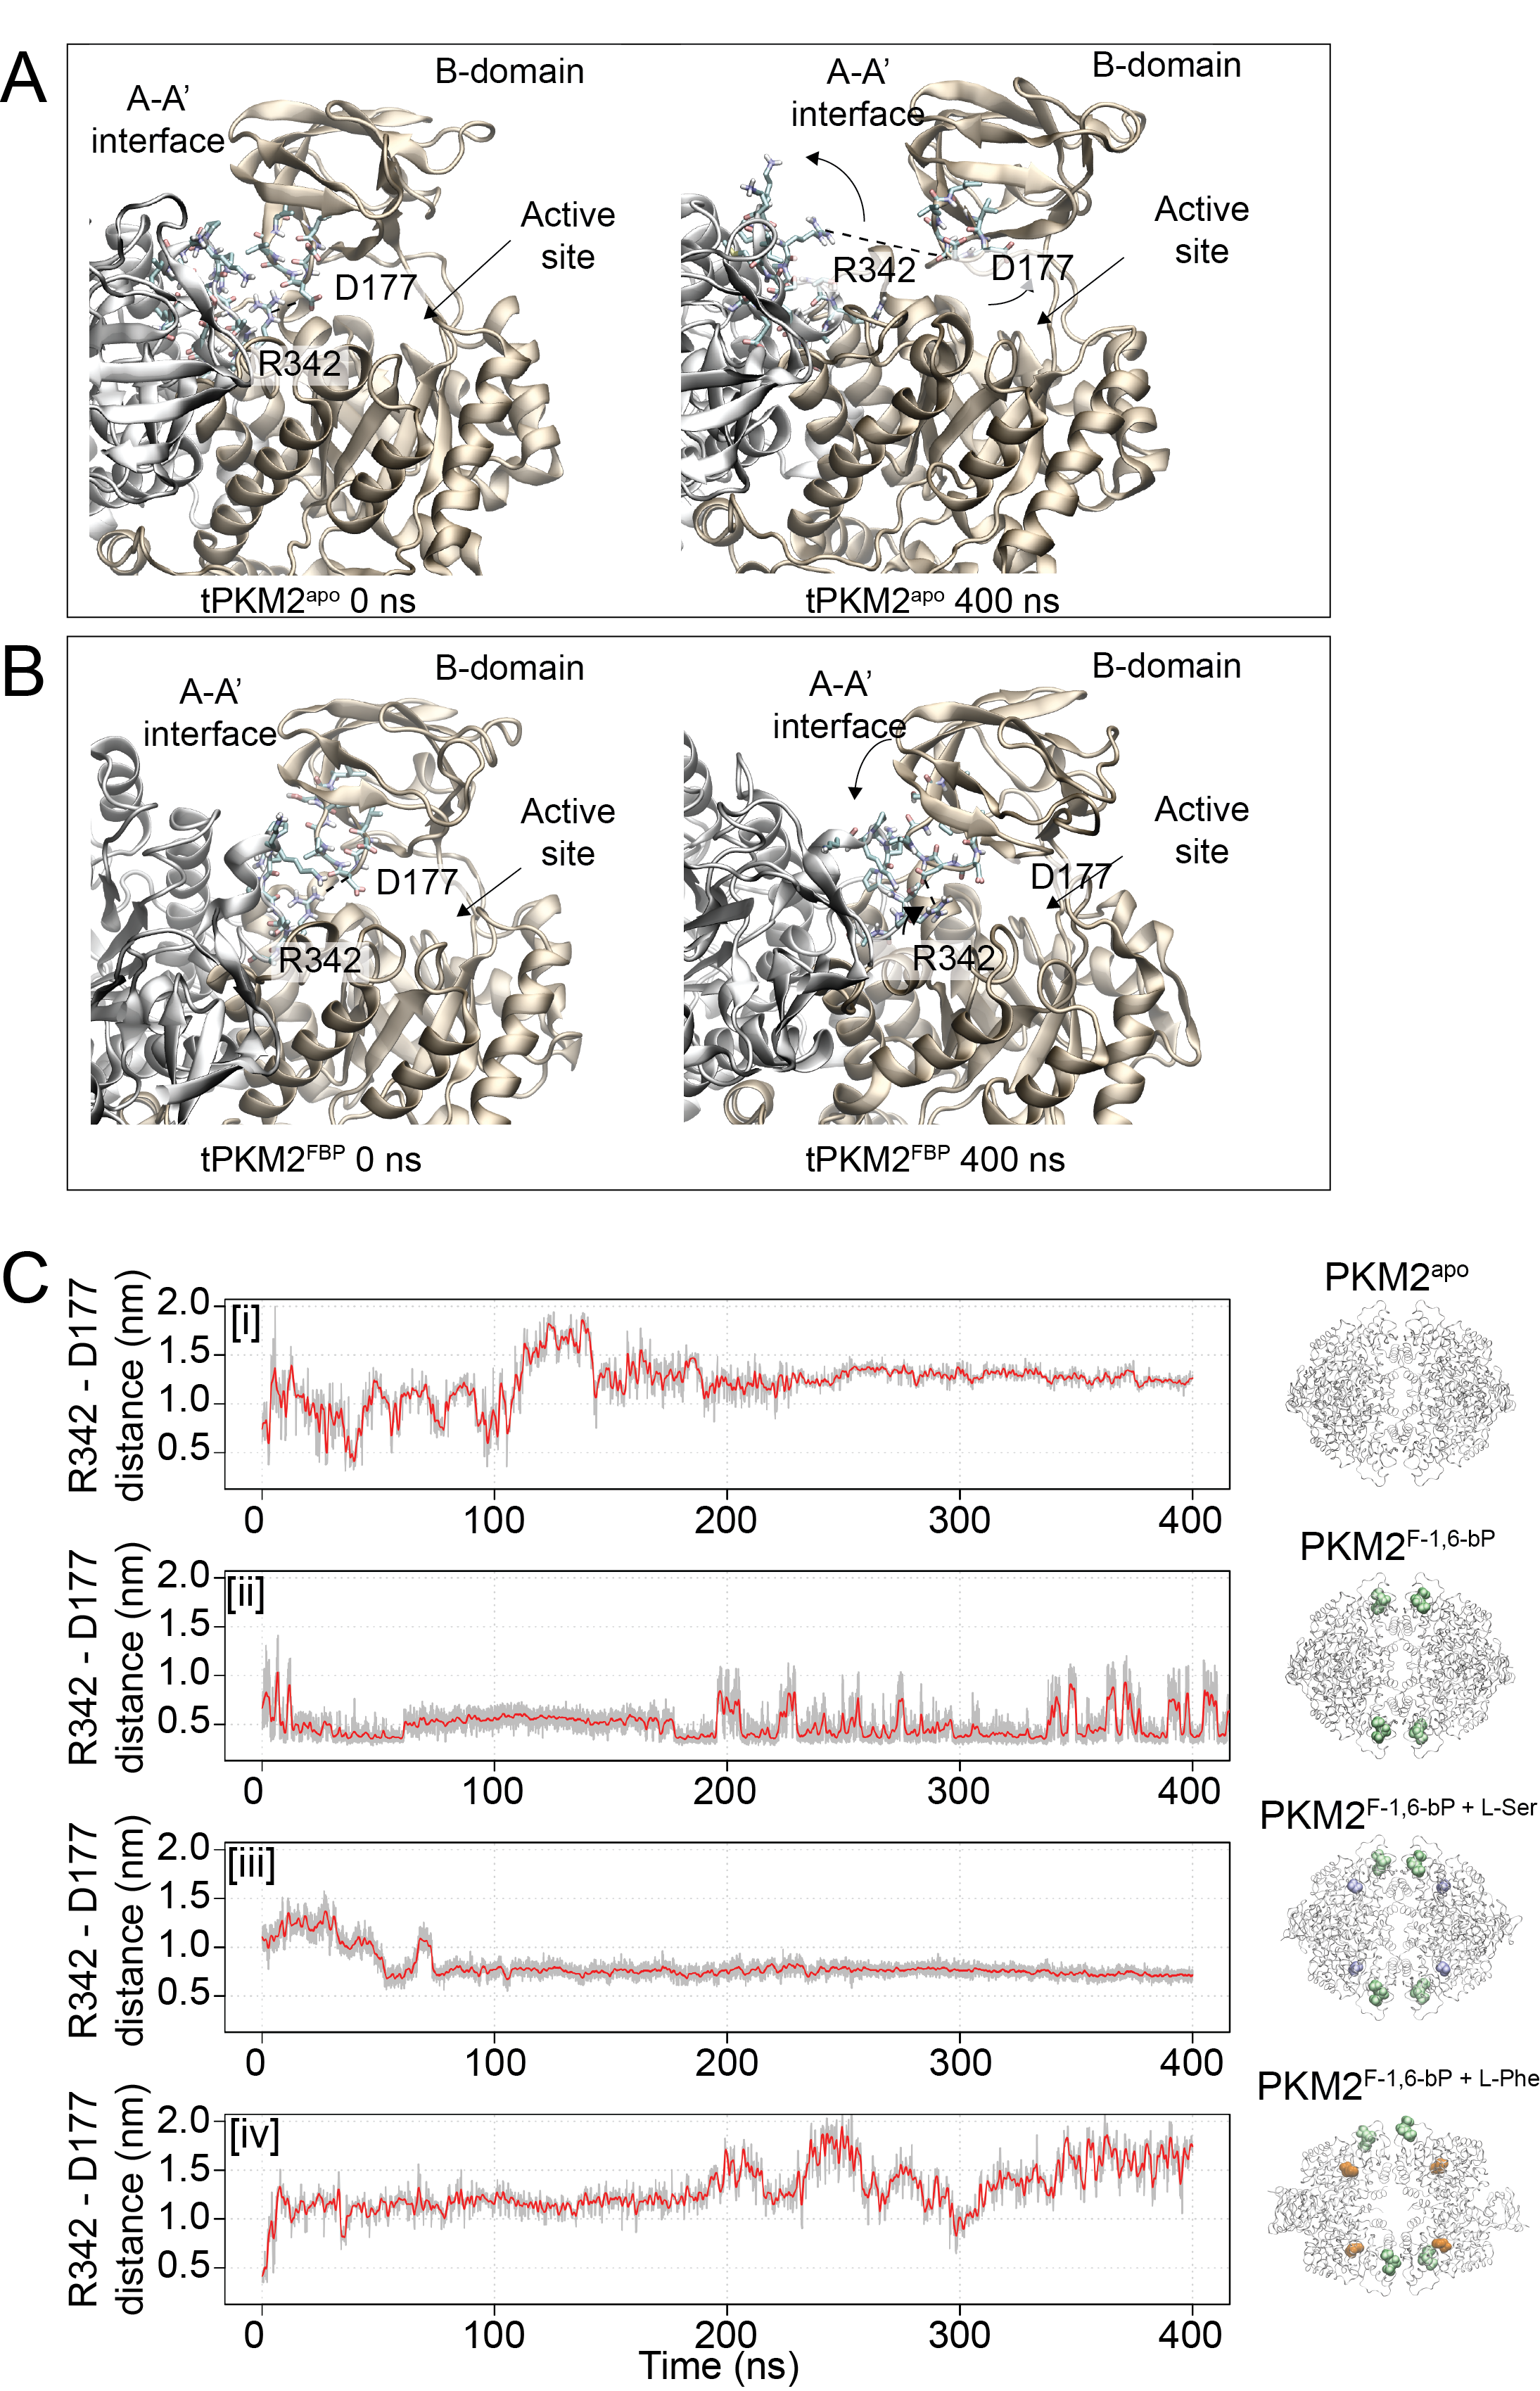
\includegraphics[scale=0.6]{ch6_fig6_tetramer_Bdomain_MD.png}
\caption[Charged-charged interactions at the A-A' interface prevent lateral B-domain closure in tetrameric PKM2.]{\textbf{Charged-charged interactions at the A-A' interface prevent lateral B-domain closure in tetrameric PKM2.} \textbf{(A)} Structures of tPKM2$^{apo}$ at 0 ns and 400 ns show that R342 and D177 flip away from the A-A' interface, breaking a crucial interface charge-charge interaction. \textbf{(B)} Structures of tPKM2$^{FBP}$ at 0 ns and at 400 ns show a tightening at the A-A' interface. \textbf{(C)} The distance between R342 and D177 about the A-A' interface is quantified for [i] tPKM2$^{apo}$, [ii] tPKM2$^{FBP}$, [iii] tPKM2$^{FBP+Ser}$ and tPKM2$^{FBP+Phe}$.}
\label{fig:tet_bdomain}
\end{figure}
%
%
\clearpage

\subsection{The configurational entropy of PKM2 does not change upon allosteric ligand binding}
\label{subsec:config_entropy}
Entropy-driven allosteric regulation has been described in a number of proteins \cite{Capdevila:2017aa,Cooper:1984aa,Popovych:2006aa,Saavedra:2018aa,Tzeng:2012aa} where, in the absence of large-scale structural changes, allosteric ligand binding modulates the amplitude of thermal fluctuations by altering the local effective elastic modulus of the protein \cite{Motlagh:2014aa}. The configurational entropy of a macromolecular system can be calculated using a formalism first proposed by Juergen Schlitter (1993) \cite{Schlitter:1993aa}, using the covariance matrix of atom-positional fluctuations. 
%
%
\\\\
%
%
The derivation of the Schlitter entropy for macromolecular systems is based on a quantum-mechanical treatment of a system with a of a one-dimensional degree of freedom $x$ with states $n$ and energies of states given by $\epsilon_{n}$. The canonical partition function is given by:
%
%
\begin{equation}
Z = \sum_{n} exp \left(- \frac{\epsilon_{n}}{k_{B}T} \right)
\end{equation}
%
%
where $k_{B}$ is the Boltzmann constant at temperature $T$. The entropy of this system can be expressed by:
%
%
\begin{equation}
S = -k_{B} \sum_{n} p_{n} \: ln \: p_{n}
\end{equation}
%
%
where $p_{n}$ is the probability of finding the system in a given state, given by:
%
%
\begin{equation}
p_{n} = \frac{exp \left( \frac{\epsilon_{n}}{k_{B}T} \right) }{Z}
\end{equation}
%
%
A single harmonic oscillator demands that the energy of a state is proportional to its variance ($\epsilon_{n} \simeq \langle n | x^2 | n \rangle$), and the complete entropy of a single harmonic oscillator is given by:
%
%
\begin{equation}
S = \frac{k_{B} \alpha}{e^{\alpha} - 1} - k_{B} \: ln \: [ 1 - e^{- \alpha}]
\end{equation}
%
%
where $\alpha = \hbar \omega \beta$, $\hbar = \frac{h}{2 \pi}$, $h$ is Plank's constant and $\omega$ is the frequency of the oscillator, which depends on the quantum-mechanically defined variance $\langle x_{2} \rangle$. For a classical system the equipartition function provides the link between the quantum-mechanically defined variance and that defined in classical mechanics. Therefore, the configurational entropy of a classical system can be given by:
%
%
\begin{equation}
S' = \frac{1}{2} k_{B} \: ln \: \left( 1 + \frac{e^{2}}{\alpha^{2}} M \sigma '_{ij} \right) 
\label{equ:schlitter_entropy}
\end{equation}
%
%
where $\sigma '_{ij}$ is the mass-weighted covariance matrix as previously defined in Equ. \ref{equ:covmat}.
%
%
\\\\
%
%
The approximative configurational entropy was calculated for all simulations of tetrameric PKM2 using Equ. \ref{equ:schlitter_entropy}, in order to \textcolor{red}{determine} whether allosteric ligands might induce an entropic change to the PKM2 structure. No significant differences in the converged configurational entropy calculated from simulated trajectories of tPKM2$^{apo}$, tPKM2$^{FBP}$, tPKM2$^{FBP+Ser}$ and tPKM2$^{FBP+Phe}$ (\textbf{Fig. \ref{fig:entropy}}), negating the likelihood of a purely entropy-driven allosteric mechanism of PKM2 regulation.
%
%
%
%
%%% FIGURE
%
\begin{figure}[!ht]
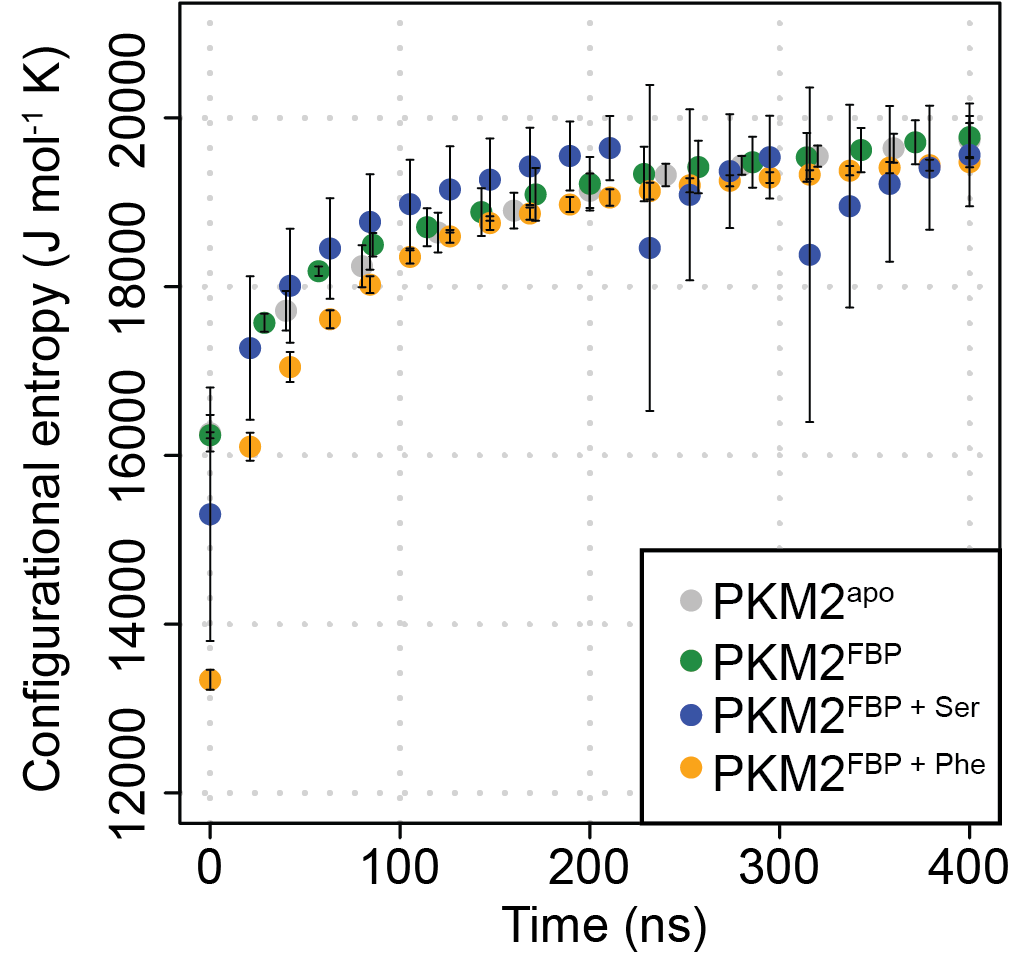
\includegraphics[scale=0.8]{ch6_fig8_entropy.png}
\caption[Allosteric ligands do not change the configurational entropy of PKM2.]{\textbf{Allosteric ligands do not change the configurational entropy of PKM2.} The time-dependent configurational entropy was computed for simulated trajectories of $tPKM2^{apo}$ (grey), $tPKM2^{FBP}$ (green), $tPKM2^{FBP+Ser}$ (blue) and $tPKM2^{FBP+Phe}$ (orange).}
\label{fig:entropy}
\end{figure}
%
%
\clearpage



\section{Identification of PKM2 allosteric hub residues using a novel software AlloHubMat}
\label{sec:allohubmat_dev}
Ligand-induced changes to the collision cross section of PKM2 (Section \ref{subsec:fbp_ccsd}) together with evidence from MD simulations of B-domain closure upon allosteric activator binding (Section \ref{subsec:tet_bdomain_closure}) suggested that backbone motions within tetrameric PKM2 contribute towards the allosteric transition of the protein. In the absence of changes to the configurational entropy of PKM2 upon ligand binding (Section \ref{subsec:config_entropy}), we hypothesised that FBP binding elicits a network of correlated motions within the backbone of PKM2, and that these concerted motions form the basis of a network of residues which connect the FBP binding pocket to the active site.
%
%
\\\\
%
%
We set out to quantify the network of correlated motions in MD simulations of PKM2 as a means for identifying residues involved in the allosteric mechanism. Particularly successful has been the the use of structural fragment analysis methods \cite{Craveur:2015aa}, and in particular the GSAtools developed by Pandini \textit{et al.} (2013) \cite{Pandini:2013aa}, which were applied towards identifing distally correlated motions in the backbone of proteins in order to elucidate allosteric pathways driven by local conformational switches \cite{Pandini:2012aa,Motta:2018aa,Pandini:2010aa,Pandini:2016aa}. The GSAtools method uses information theory to compute the normalised mutual information (nMI) between each fragment-encoded position in the protein (Section \ref{subsec:discrete_state_mi}). Given that each element in the nMI matrix has a time component, the network of correlated motions is likely to change over the simulated time. In this context, the time-evolution of correlated motions derived from an information theoretical treatment of the protein structure has never been explored. Moreover, no methods had been previously developed to allow for the comparison of nMI matrices extracted from multiple replicate MD trajectories.
%
%
\\\\
%
%
We therefore developed a novel computational framework, named AlloHubMat (\textbf{Allo}steric \textbf{Hub} prediction using \textbf{Mat}rices that capture allosteric coupling), to predict allosteric hub fragments from the network of dynamic correlated motions, based on explicitly identified conformational sub-states from multiple MD trajectories (\textbf{Fig. \ref{fig:allohubmat_schematic} A}). Extraction of correlated motions from multiple sub-states within a consistent information theoretical framework allowed us to compare the allosteric networks, both between replicas of the same liganded state and between different liganded states of PKM2. To automate the prediction of allosteric hub residues from MD trajectories, AlloMatHub was implemented as a stand-alone R package (\textbf{Fig. \ref{fig:allohubmat_schematic} B}). Here, the core functionalities of AlloHubMat will be described, followed by a discussion of how the method was used to identify allosteric residues in PKM2.
%
%
%
%
%%% TABLE
% Please add the following required packages to your document preamble:
% \usepackage{booktabs}
\begin{table}[]
\centering
\caption{Available functions contained within the R package AlloHubMat1.0}
\label{tab:allomathub_functions}
\begin{tabular}{@{}ll@{}}
\toprule
Function           								& Description                                                                              												\\ \midrule
read\_pdb\_file()          					& Read PDB topology file.                                             															\\
read\_traj\_file()							& Read DCD MD trajectory file.										  															\\
superpose\_trj()							& Remove roto-translational motion from MD trajectory.													\\
encode\_dcd\_trajectory()    		& Encode trajectory with the M32K25 structural alphabet.              			                       \\
split\_sa\_align()   						& Split the structural alphabet alignment into regular blocks.                                          \\
mi\_mat()										& Compute the mutual information matrix.																				 \\
comp\_eigensystem()    		        & Compute the eigen system of the mutual information matrix.                      			     \\
block\_overlap()         					& Compute the covariance overlap between each mutual 													  \\
 & information matrix.				 \\                 
matrix\_smooth()   					    & Linear smoothing of the covariance overlap blocks.                               						   \\
detect\_sectors()						    & Detection of conformational sub-states.                                             									\\
extract\_sectors()  					    & Extract mutual information for each conformational sub-state.                    				   \\
allosteric\_path()  						& Minimal distance pathfinder between allosteric and active sites.                    					\\
identify\_hubs()   						    & Identify allosteric hub residues.                                        											           \\
sectors\_2dplot()   						& Plot the covariance overlap of time-contiguous covariance overlap.                  			\\
sectors\_3dplot()   						& Plot the covariance overlap of all combinations of time-blocked										\\
&  covariance overlap. \\ \bottomrule
\end{tabular}
\end{table}
%
%
%
%
%%% FIGURE
%
\begin{figure}[!ht]
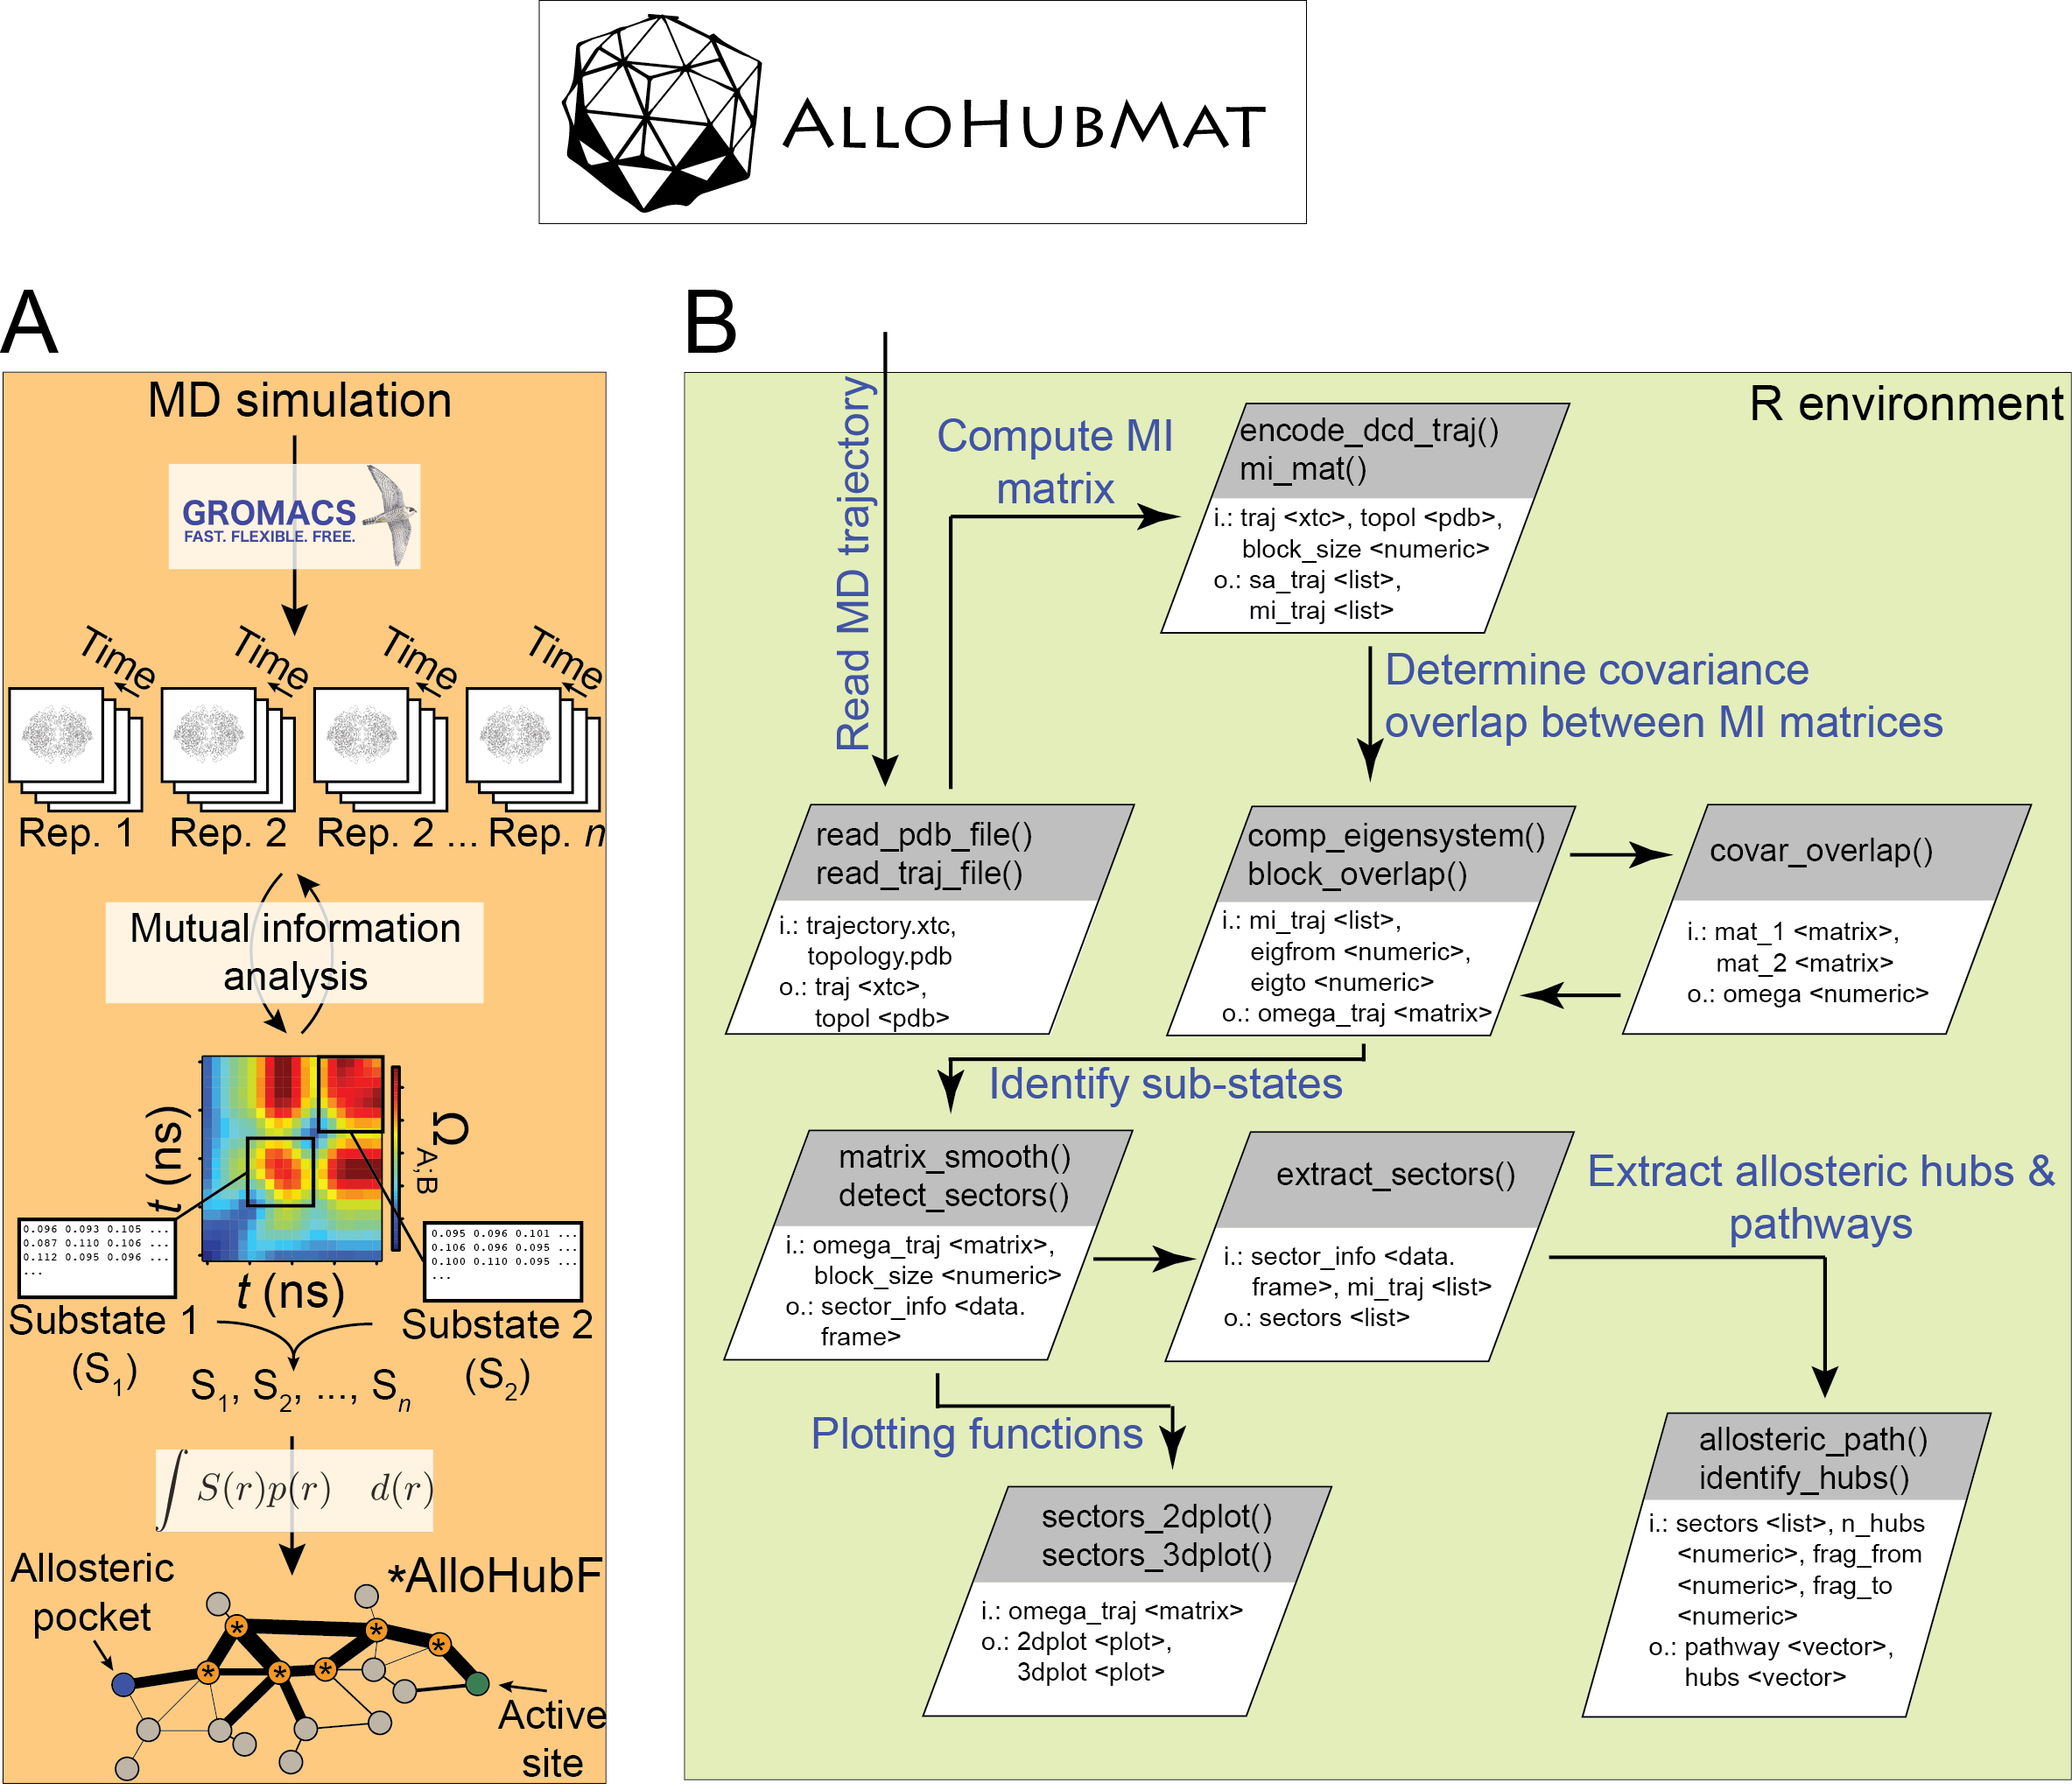
\includegraphics[scale=0.7]{ch6_fig9_software_diag.png}
\caption[Schematic of the AlloHubMat and software flowchart.]{\textbf{Schematic of the AlloHubMat and software flowchart.} \textbf{(A)} Multiple replicate molecular dynamics (MD) simulations are calculated using the GROMACS molecular dynamics engine \cite{Van-Der-Spoel:2005aa}. All MD simulations are encoded with the M32K25 structural alphabet \cite{Pandini:2010aa}, and the strength of dynamic protein backbone correlations over the MD trajectory is computed using information theory mutual information statistics. The backbone correlations are explicitly used to identify and extract configurational sub-states from the MD trajectories. A global allosteric network is then constructed by integrating over the correlation matrices, and their respective probabilities, from which allosteric hub (AlloHub) fragments are extracted. AlloHub fragments are overlapping regions of four consecutive amino acid residues. \textbf{(B)} A software flowchart of AlloMatHub showing the functionalities of the software.}
\label{fig:allohubmat_schematic}
\end{figure}
%
%
\clearpage


\subsection{Explicit identification of sub-states from MD simulations using information theory}
Correlated motions have demonstrated as important towards protein dynamics and allostery. To extract correlated motions from MD trajectories, an information theoretical framework was used based on a coarse-grained representation of the protein backbone conformation with the M32K25 structural alphabet \cite{Pandini:2010aa}, as previously described (Section \ref{subsec:discrete_state_mi}). 
%
%
\\\\
%
%
MD trajectories of tPKM2$^{apo}$, tPKM2$^{FBP}$, tPKM2$^{FBP+Ser}$ and tPKM2$^{FBP+Phe}$ were sub-divided into 20 non-overlapping blocks with an equal time length of 20 $ns$ each. For each block, the normalised mutual information between distal backbone-encoded fragments $\left[ I^{n}(C_i; C_j) \right]$ was calculated for all pairs of fragments $(i,j)$:
%
%
\begin{flalign}
I^{n}_{B}(C_i; C_j) = \frac{I_{B}(C_i; C_j) - \epsilon_{B} (C_i; C_j)}{H_{B}(C_i, C_j)}
\label{equ:norm_mutual_information}
\end{flalign}
%
%
where the columns of the structural fragment alignment are given by $C_i$ and $C_j$, $I(C_i; C_j)$ is the mutual information, $\epsilon(C_i; C_j)$ is the expected finite size error and $H(C_i, C_j)$ is the joint entropy (see Section \ref{subsec:discrete_state_mi} for a full derivation of the individual terms of the equation). \textcolor{red}{The normalised mutual information $I^{n}_{B}(C_i; C_j) $ has a range between 0 and 1. Two independent, random distributions would have a normalised mutual information score of 0, whereas two identical distributions would have a normalised mutual information equal to 1. Therefore, two fragments with a normalised mutual information approaching 1  indicates that these two fragments are correlated in their motion throughout the simulation. In contrast, two fragments with a normalised mutual information approaching 0 reveals that these two fragments are uncorrelated in their motion.}
%
%
\\\\
%
%
With the goal of identifying conformational sub-states from a time-trajectory of mutual information matrices, eigenvalue decomposition was used to compute the geometric evolution of the protein backbone correlations. The elements of the mutual information matrix are proportional to the square of the displacement, so the square root of the matrix is required to examine the extent of the matrix overlap:
%
%
\begin{flalign}
d(A,B) &= \sqrt{tr[(A^{\frac{1}{2}} - B^{\frac{1}{2}} )^2 ]} && \\
&= \sqrt{tr[A + B -2A^{\frac{1}{2}} B^{\frac{1}{2}} ]} &&\\
&= \sqrt{\sum^{3N}_{i=1} (\lambda_{i}^{A} + \lambda_{i}^{B}) - 2 \sum^{3N}_{i=1} \sum^{3N}_{j=1} (\lambda_{i}^{A} \cdot \lambda_{j}^{B})^{\frac{1}{2}} (\textbf{v}_{i}^{A} \cdot \textbf{v}_{j}^{B})^2} &&\\
\Omega_{A;B} &= 1 - \frac{d(A,B)}{\sqrt{tr A + tr B}} 
\label{equ:covariance_overlap}
\end{flalign}
%
%
where $\lambda^A$ and $\lambda^B$ denote the eigenvalues and $\textbf{v}^A$ and $\textbf{v}^B$ the eigenvectors of mutual information matrices A and B, $N$ is the number of fragments used to encode the polypeptide chain. The covariance matrix overlap ($\Omega$) ranges from $0$ when matrices A and B are orthogonal, and $1$ when they are identical. 
%
%
\\\\
%
%
The geometric difference between any two mutual information matrices, with identical dimensions, could be numerically compared by calculating the covariance overlap between the mutual information from time-contiguous trajectory blocks:
%
%
\begin{equation}
\Omega_{B;B-1} = 1 - \frac{ d \left[ I^{n}_{B}(C_{i}; C_{j}) -  I^{n}_{B-1}(C_{i}; C_{j}) \right] }{ \sqrt{ tr \left[ I^{n}_{B}(C_{i}; C_{j}) \right] + tr \left[ I^{n}_{B-1}(C_{i}; C_{j}) \right] } }
\label{equ:omega_mi_blocks}
\end{equation}
%
%
The covariance matrix overlap between each time-contiguous mutual information matrix (Equ. \ref{equ:omega_mi_blocks}) revealed an oscillatory similarity in the nMI over time (\textbf{Fig. \ref{fig:cov_overlap_trj} A} and \textbf{B}). For some regions of the MD trajectories the nMI matrices were very self-similar, reflected by $\Omega_{B;B-1} > 0.2$, suggesting that the protein was sampling a local sub-state. Conversely, other regions of the MD trajectories contained nMI matrices which were very different from the previous time block ($\Omega_{B;B-1} \rightarrow 0$), implying non-ergodic sampling. Sub-states were heuristically defined as regions which displayed $\Omega_{i}$ values in the top quartile (\textbf{Fig. \ref{fig:cov_overlap_trj} C} and \textbf{D}). The mutual information was averaged for each unique sub-state identified from a given trajectory, for further analysis. 
%
%
%
%
%%% FIGURE
%
\begin{figure}[!ht]
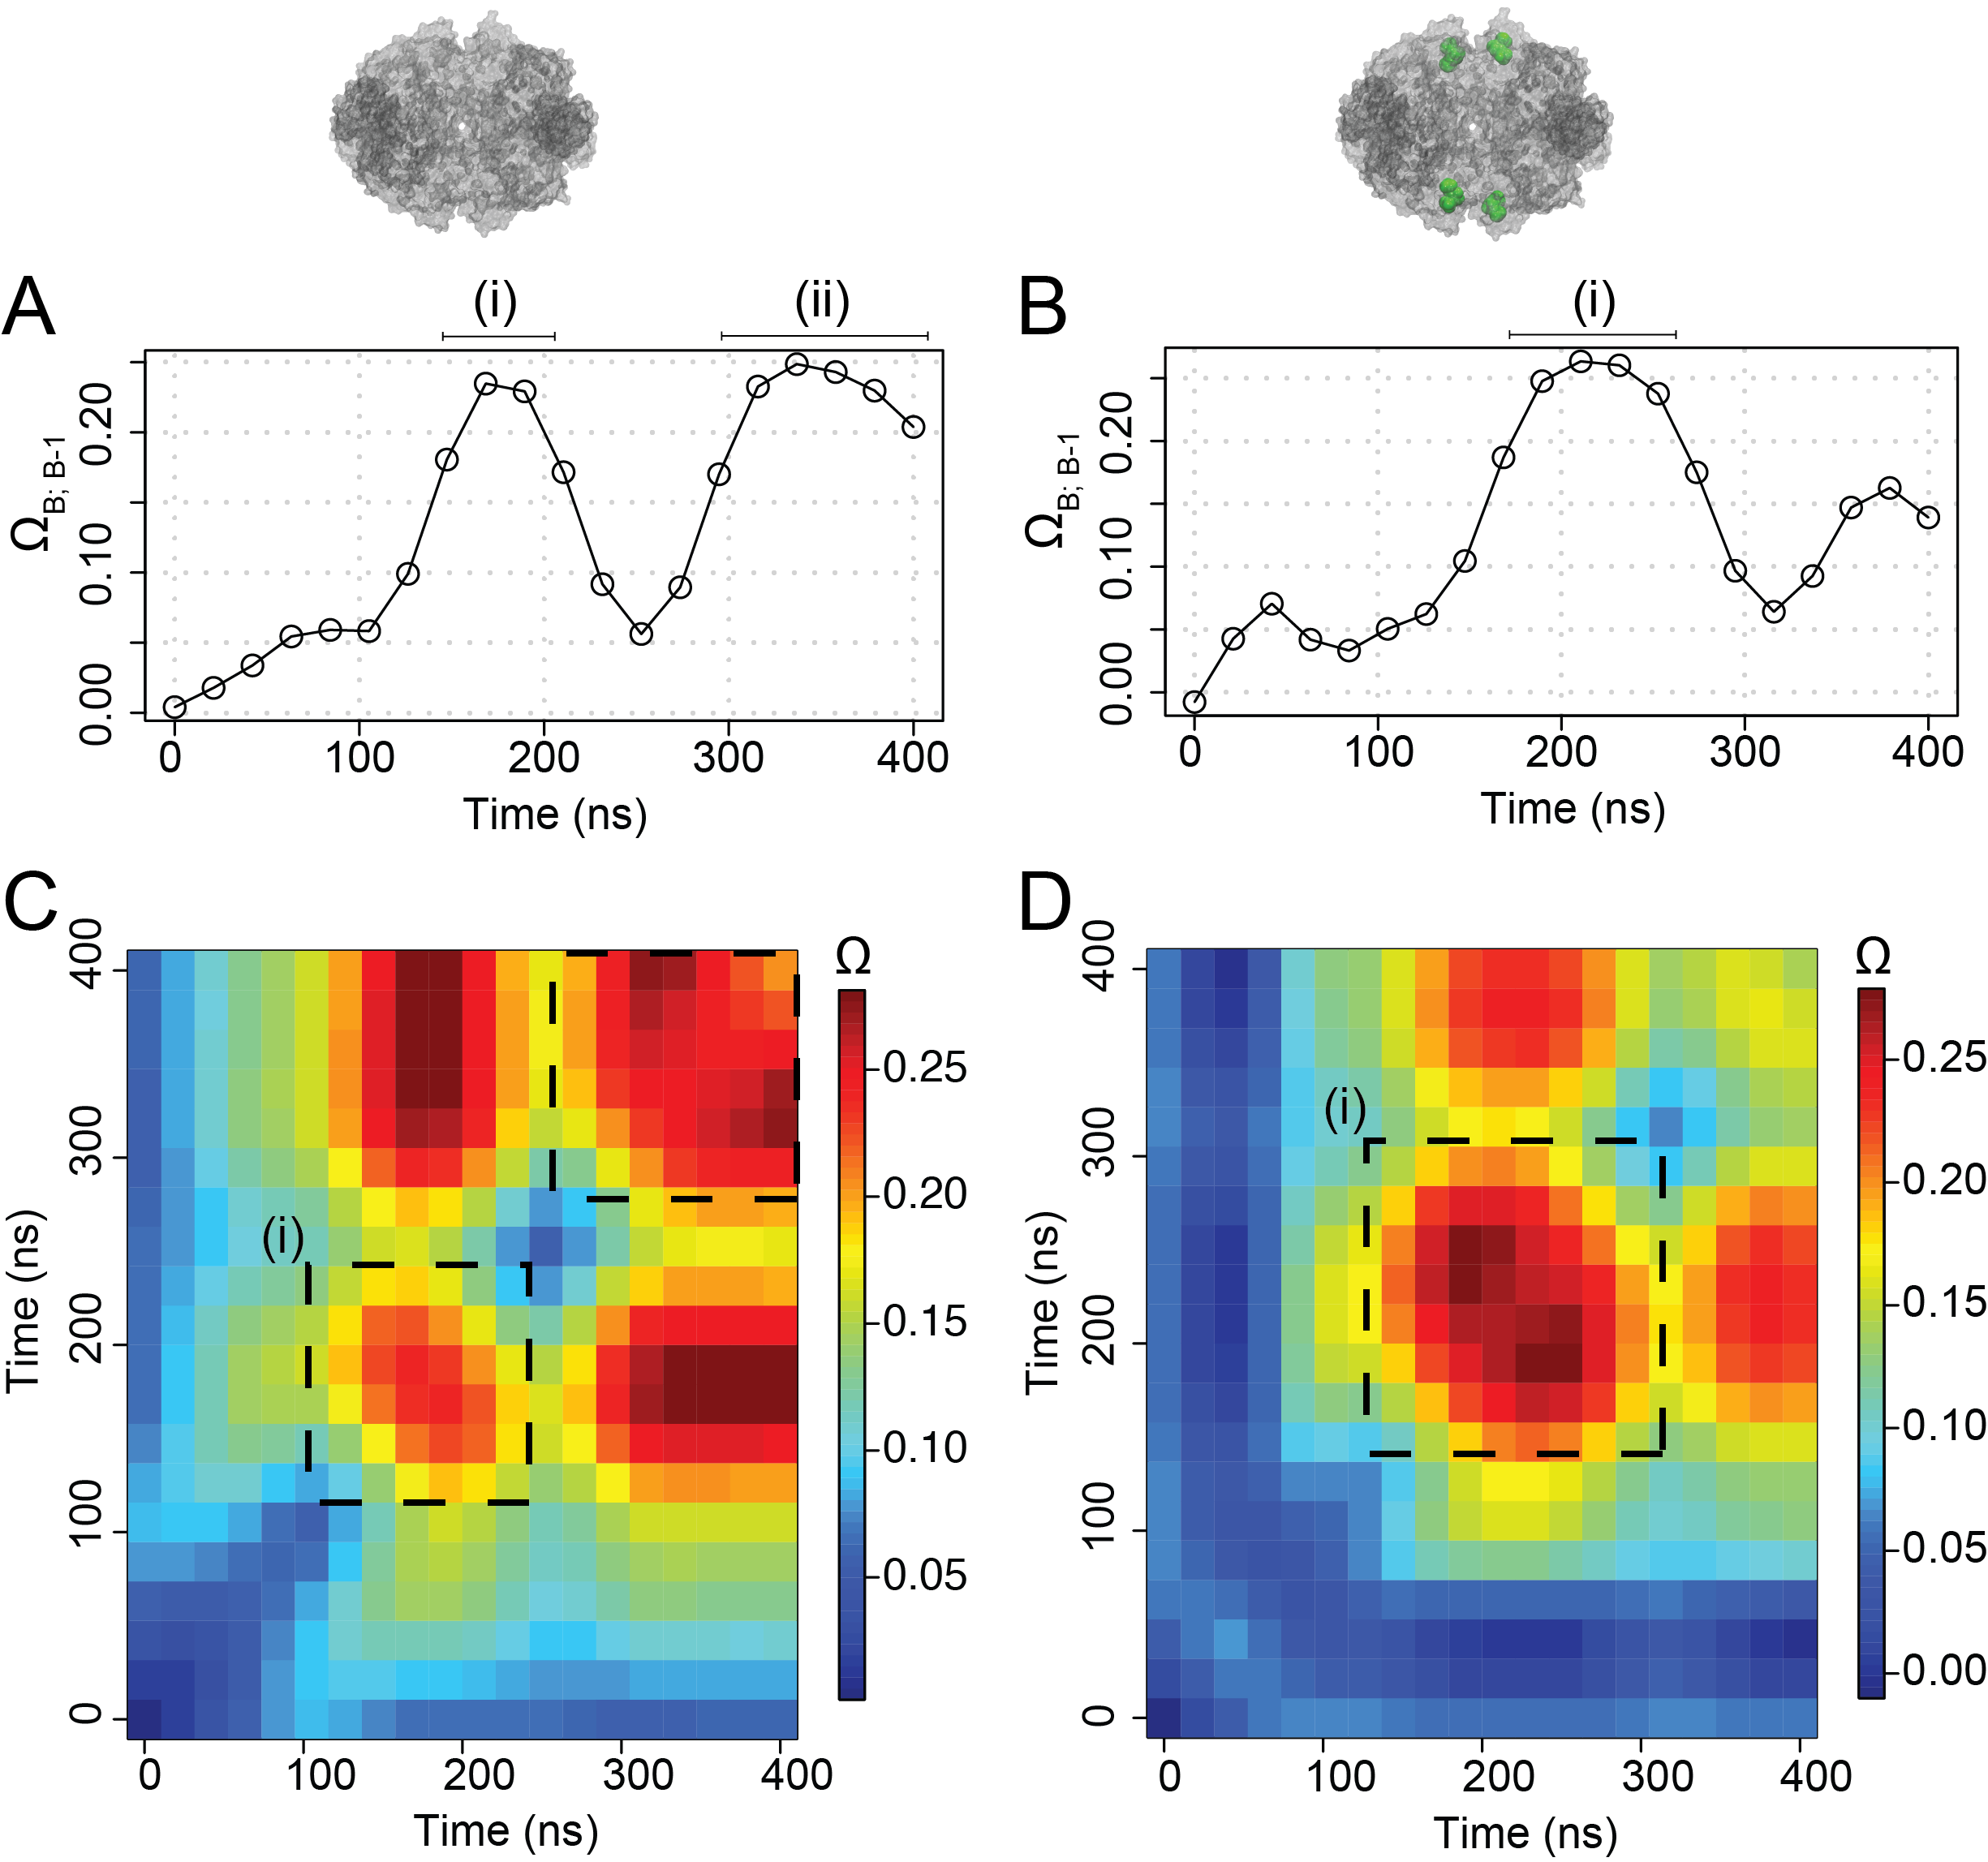
\includegraphics[scale=0.7]{ch6_fig10_omega_traj.png}
\caption[Conformational sub-states are identified from the geometric progression of the mutual information matrix.]{\textbf{Conformational sub-states are identified from the geometric progression of the mutual information matrix.} The time-dependent matrix covariance overlap between contiguous mutual information matrices computed from contiguous trajectory blocks is quantified using Equ. \ref{equ:omega_mi_blocks} for an example replica of \textbf{(A)} tPKM2$^{Apo}$ and \textbf{(B)} tPKM2$^{FBP}$. The matrix covariance overlap was computed for all combinations of time-resolved nMI blocks. The resulting matrices were smoothed and are shown for example replicate MD simulations of \textbf{(C)} tPKM2$^{apo}$ and \textbf{(D)} tPKM2$^{FBP}$. Sub-states were identified as regions containing a covariance overlap in the top quartile of the trajectory (shown as dashed boxes).}
\label{fig:cov_overlap_trj}
\end{figure}
%
%
\clearpage

\subsection{PKM2 sub-states cluster according to the liganded state of the MD simulation}
A total of 7 substates were identified for all MD simulations of tPKM2$^{apo}$, 6 for tPKM2$^{FBP}$, 4 for tPKM2$^{FBP+Ser}$ and 3 for tPKM2$^{FBP+Phe}$. To investigate whether the correlated motions for each sub-state could be attributed to the liganded state of the MD simulation, the mutual information matrices extracted from each unique sub-state were compared with a complete-linkage hierarchical clustering, using the covariance matrix overlap in Equ. \ref{equ:covariance_overlap} as a distance metric (\textbf{Fig. \ref{fig:mi_cluster}}). Clustering of the sub-states revealed four predominant clusters (denoted as \textit{C1} - \textit{C4}). nMI matrices from tPKM2$^{apo}$ were found to predominate in cluster 1, tPKM2$^{FBP}$ in cluster 2 and tPKM2$^{FBP+Ser}$ in cluster 3. We found cluster 4 to be populated by both tPKM2$^{apo}$ and tPKM2$^{FBP+Phe}$, as well as a number of tPKM2$^{FBP}$ replicas.
%
%
\\\\
%
%
The commonality between the sub-state mutual information matrices of the same liganded state suggested that each of the replicate MD simulations converged to a common sub-state, which was ligand-dependent. Moreover, this suggested that allosteric ligand-dependent correlated motions were captured by the preceding analysis. Therefore, an ensemble-averaged nMI matrix was computed for PKM2 in each of the four liganded states, as an integral over all sub-states ($I^{n}_{ss}$) of the protein ($r$) weighted by the probability of the sub-state ($p$):
%
%
\begin{equation}
\langle I^{n}_{ens} \rangle = \int I^{n}_{ss} \: p(r) \quad dr
\end{equation}
%
%
%
%
%%% FIGURE
%
\begin{figure}[!ht]
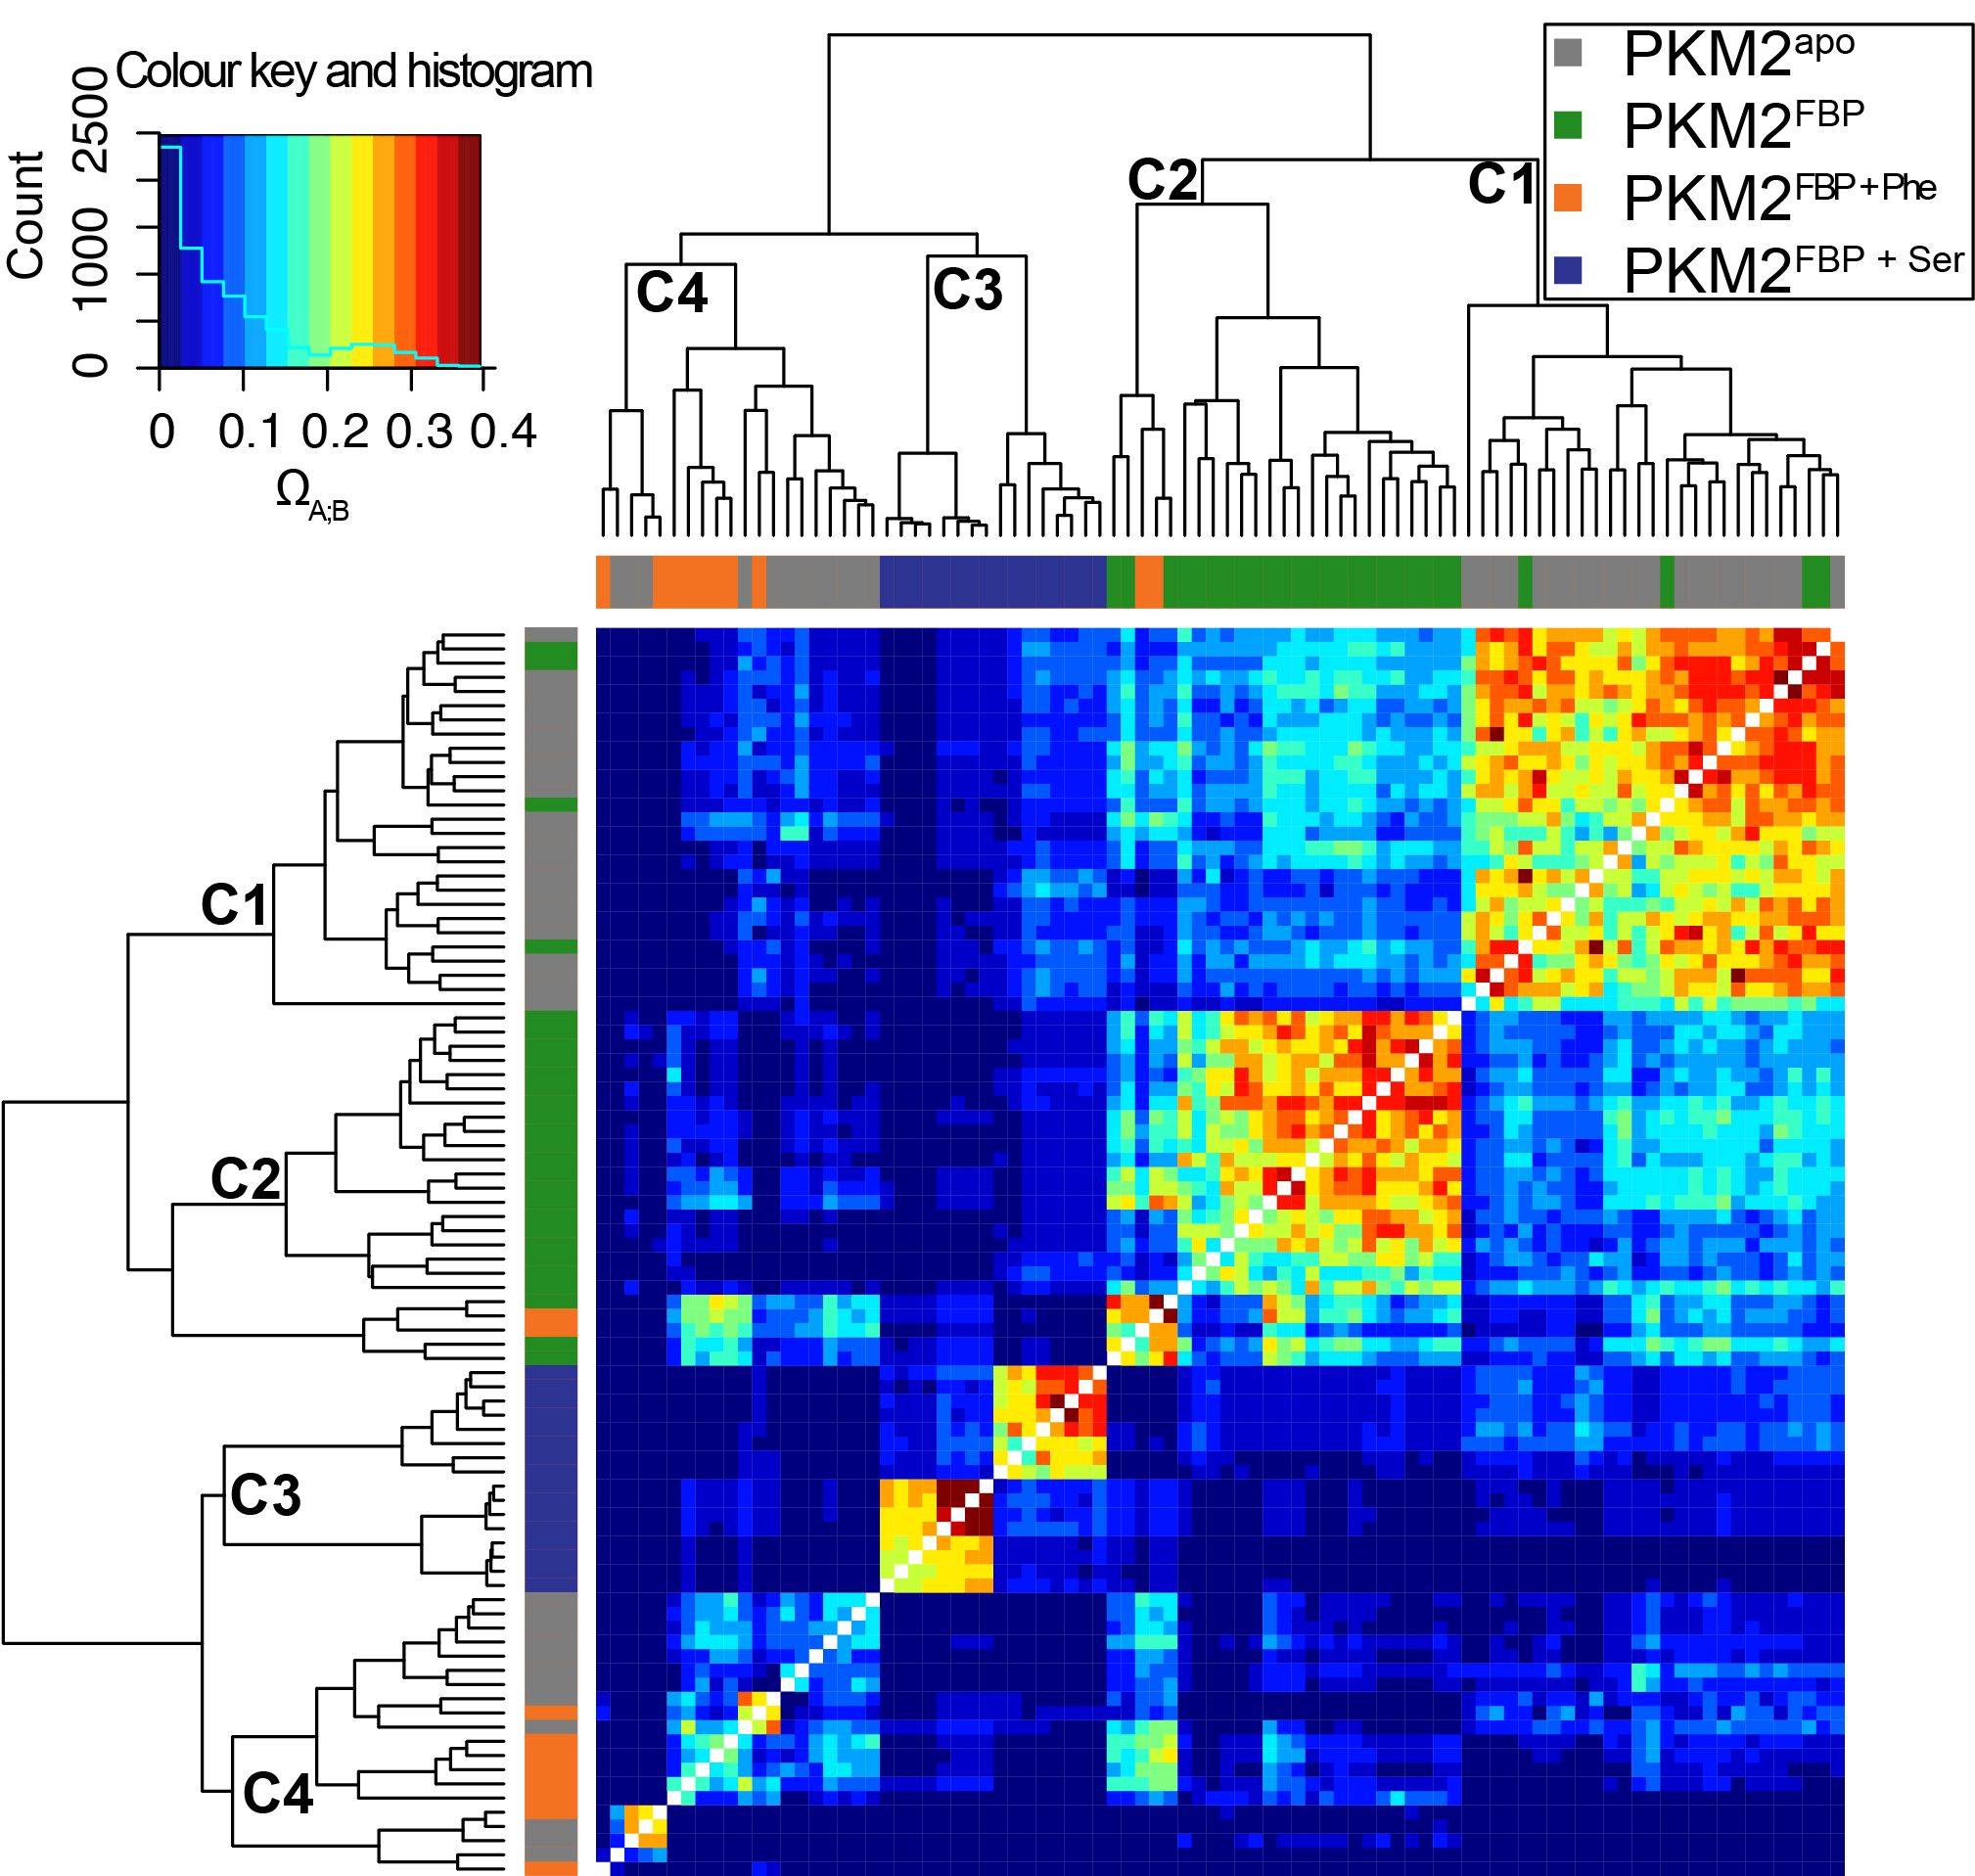
\includegraphics[scale=0.7]{ch6_fig11_substate_cluster.png}
\caption[PKM2 correlated motions cluster according to the liganded state of the simulation.]{\textbf{PKM2 correlated motions cluster according to the liganded state of the simulation.} A complete-linkage hierarchical clustering of mutual information matrices, computed from simulated trajectories of $tPKM2^{apo}$ (grey), $tPKM2^{FBP}$ (green), $tPKM2^{FBP+Ser}$ (blue) and $tPKM2^{FBP+Phe}$ (orange). Four clusters are assigned C1 - C4. For every sub-state, the network of correlations from each of the four protomers is presented individually.}
\label{fig:mi_cluster}
\end{figure}
%
%
\clearpage



\subsection{A disperse network of hub residues are predicted to propagate FBP-induced activation of PKM2}
\label{subsec:allohubfrag_ident}
The ensemble-averaged matrix of correlated motions identified from the analysis of tPKM2$^{apo}$ were subtracted from those of tPKM2$^{FBP}$ to isolate the fragment positions predicted to be involved in the allosteric state transition, which were termed allosteric hub fragments (AlloHubFrags). An inspection of the frequency distribution of the mutual information matrices of tPKM2$^{apo}$ and tPKM2$^{FBP}$ found that the strength of the fragment correlations were log-normally distributed with a large Gaussian component, and a long tail to the distribution (\textbf{Fig. \ref{fig:mi_stats} A} and \textbf{B}). Subtracting the mutual information matrices resulted in the z-transformation of the distribution of correlations, with a mean $\mu_{I^{n}} = 0$ and a standard deviation $\sigma _{I^{n}} = 0.04$ (\textbf{Fig. \ref{fig:mi_stats} C}). 
%
%
\\\\
%
%
The variance of each of the \textcolor{red}{2119740} individual backbone couplings were computed within the multiple conformational sub-states for tPKM2$^{apo}$ and tPKM2$^{FBP}$. We found that when the average difference in the mutual information between the two liganded states ($\mu \Delta^{FBP}$) was inspected against the variance of each of the couplings ($\sigma \Delta^{FBP}$), the resulting plot formed a v-shape with highly correlated fragments showing a high degree of variance (\textbf{Fig. \ref{fig:mi_stats} D}). 
%
%
%
%
%%% FIGURE
%
\begin{figure}[!ht]
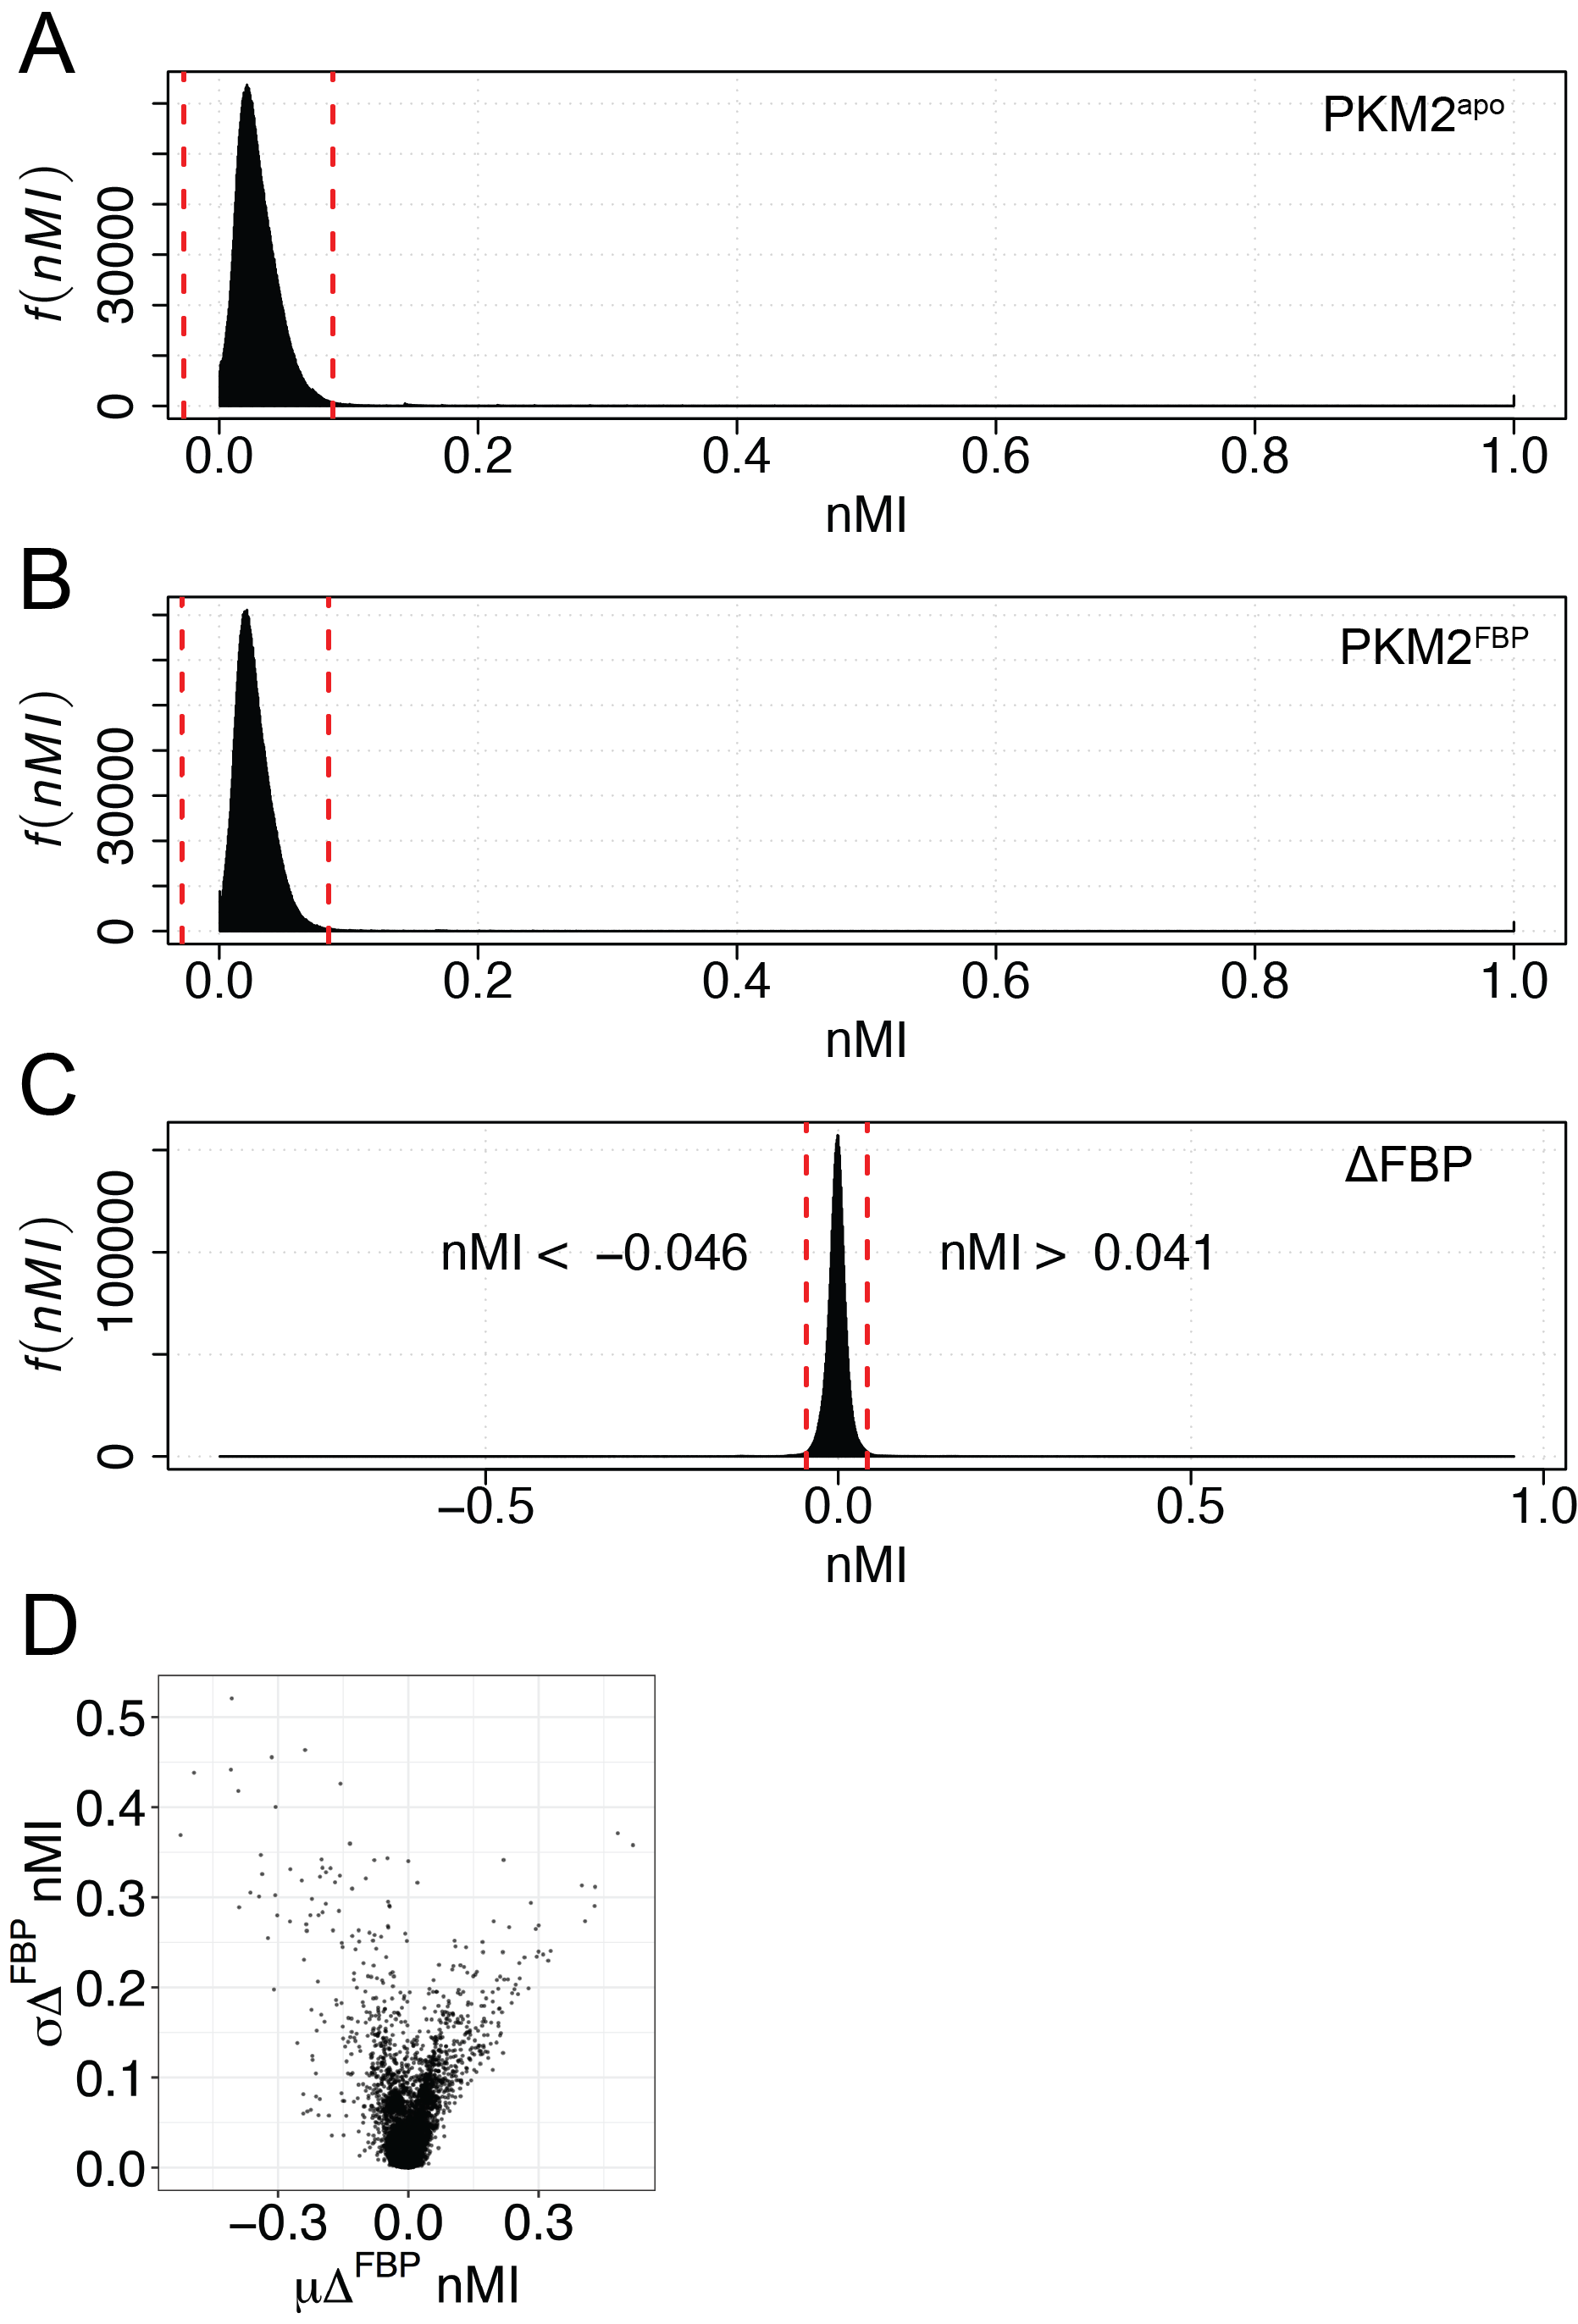
\includegraphics[scale=0.7]{ch6_fig12_MI_stats.png}
\caption[The sub-state mutual information matrix is log-normally distributed.]{\textbf{The sub-state mutual information matrix is log-normally distributed.} The distribution of mutual information couplings for the ensemble-averaged mutual information matrices of \textbf{(A)} $tPKM2^{apo}$, \textbf{(B)} $tPKM2^{FBP}$, and \textbf{(C) }the subtracted mutual information matrices of the preceding two liganded states. \textbf{(D)} The variance of each coupling was computed over each of the multiple conformational sub-states, for each fragment coupling.}
\label{fig:mi_stats}
\end{figure}
%
%
\clearpage


Rather than ranking fragment positions by their nMI score, the significance of the change in nMI was computed for each coupling (\textbf{Fig. \ref{fig:allohub_identification} A}). From a total of 76 fragments identified as significant, the top AlloHubFrags were selected for further analysis ($Hubs_{1-10}$). $Hub_{5}$ and $Hub_{6}$ were found to overlap with a two amino acid residue difference between the two hubs. The AlloHubFrags were found to be spatially diverse across the PKM2 structure, though not obviously structurally contiguous (\textbf{Fig. \ref{fig:allohub_identification} B}). $Hub_{5}$ and $Hub_{6}$ were proximal to the A-A' interface, $Hub_{9}$ was proximal to the FBP binding pocket, $Hub_{10}$ localised to the C-C' interfaces and $Hub_{1}$ and $Hub_{2}$ were in the B-domain (\textbf{Fig. \ref{fig:allohub_identification} B}).
%
%
\\\\
%
%
The subtracted mutual information matrix was next distance-weighted using the C$\alpha$ distance matrix ($M$) determined from the PKM2 crystal structure:
%
%
\begin{equation}
I^{n}(C_i; C_j)' = I^{n}(C_i; C_j) \cdot \frac{1}{M}
\end{equation}
%
%
Re-weighting the mutual information matrix with the inverse of the distance matrix had the effect of down-weighting long-distance correlations and up-weighting short-range correlation, along which non-bonded chemical interactions could occur. From the distance-weight mutual information matrix, minimal distance pathways between FBP binding-pocket fragments and active-site fragments were computed using the Dijkstra algorithm in order to predict the allosteric pathways elicited by FBP. This analysis revealed that all AlloHubFrags, with the exception of $Hub_5$ and $Hub_6$, were connected to the predicted pathways (\textbf{Fig. \ref{fig:allohub_identification} B}), supporting the hypothesis that the AlloHubFrags propagate the allosteric effect of FBP.
%
%
\\\\
%
%
Of the 40 residues within the top ten-ranked AlloHubFrags, we sought to rationally guide the selection of a number of residues for experimental mutagenesis. Each fragment used to encode the backbone conformation of the MD trajectories of PKM2 is a collection of four contiguous residues, and as such, the mutual information between two fragments could not be readily assigned to an individual amino acid residue. Nevertheless, the chain rule for mutual information states that the mutual information of a collection of random variables is the sum of the conditional mutual informations:
%
%
\begin{equation}
I(X_{1}, X_{2}, ..., X_{n}; Y) = \sum_{i=1}^{n} I(X_{i}; Y | X_{i-1}, X_{i-2}, ..., X_{1}) 
\label{equ:chain_rule_MI}
\end{equation}
%
%
Assuming that the variables $X_{1}, X_{2}, ..., X_{n}$ are random, it would be possible to reconstruct the per-residue mutual information and thus select top-ranked residues with high mutual information content for mutagenesis. The validity of this assumption was tested by computing the distribution of mutual information between neighbouring fragments (\textbf{Fig. \ref{fig:allohub_identification} C}). We observed a distribution of mutual information between neighbouring fragments, which was skewed towards higher values, when compared to the same log-normal distribution of the entire mutual information matrix, suggesting that the majority of neighbouring fragments were correlated and were non-random. This proved that the underlying assumption of Equ. \ref{equ:chain_rule_MI} did not hold. Thus, it was not possible to numerically assign a per-residue mutual information score.
%
%
%
%
%%% FIGURE
%
\begin{figure}[!ht]
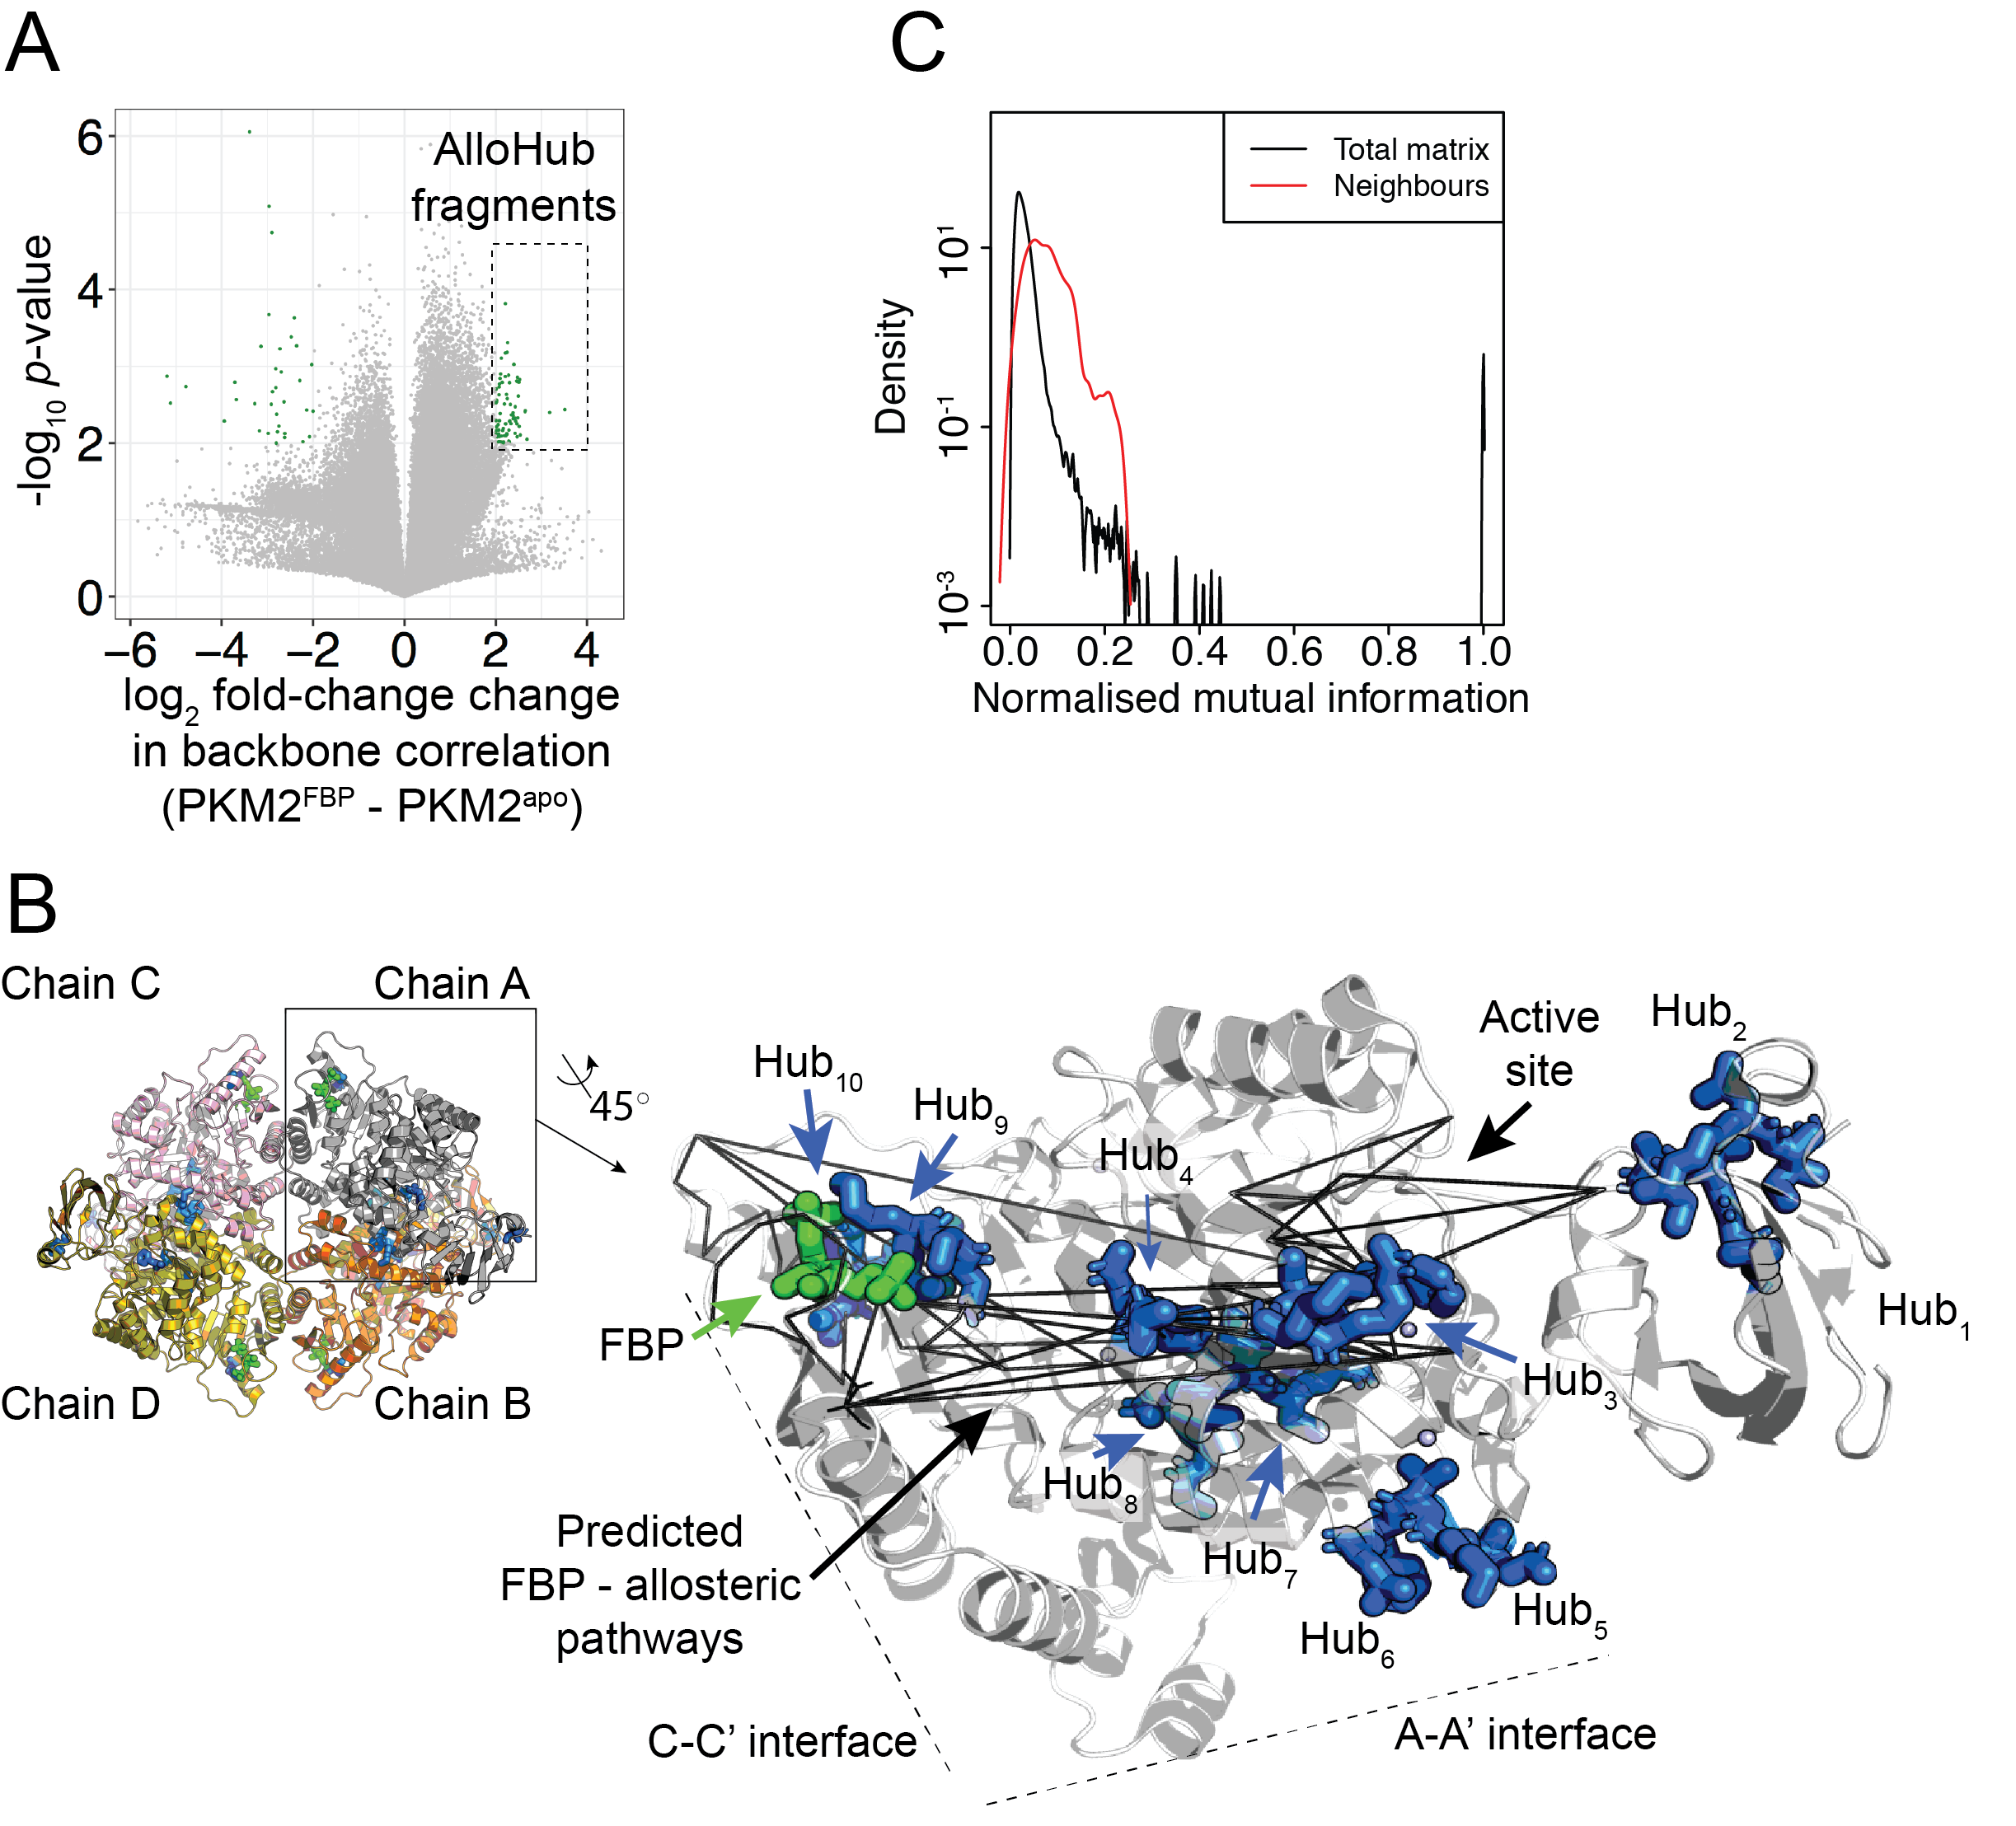
\includegraphics[scale=0.7]{ch6_fig13_allofraghubs.png}
\caption[Hub residues are predicted to propagate energy transfer along allosteric pathways.]{\textbf{Hub residues are predicted to propagate energy transfer along allosteric pathways.} \textbf{(A)} A volcano plot showing the difference in mutual information couplings between $tPKM2^{apo}$ and $tPKM2^{FBP}$. \textbf{(B)} The spatial distribution of the top ten predicted AlloHubFrags projected onto a cartoon representation of PKM2. Predicted allosteric pathways between the FBP binding pocket and the active site are shown as black lines. \textbf{(C)} The distribution of normalised mutual information for all fragment combinations (black) and for neighbouring fragments (red).}
\label{fig:allohub_identification}
\end{figure}
%
%
\clearpage

\subsection{Design of allosteric hub mutants (AlloHubMs)}
In lieu of an analytic solution to the per-residue mutual information, allosteric hub mutants (AlloHubMuts) were generated by substituting AlloHubFrag residues with amino acids that were predicted to be tolerated at the respective position based on their occurance in a multiple sequence alignment of 5381 pyruvate kinase homologues. Of the residues within the top-ten AlloHubFrags, there was variability in the degree of sequence conservation. $Hub_7$ and $Hub_8$  contained several highly conserved hydrophobic residues on parallel $\beta$-sheets within the A-domain of the protein. Of these V324, I325, A327, G355 and D357 were found to be very highly conserved within the alignment (\textbf{Fig. \ref{fig:allohub_design} A}). Conversely, residues R489 - F492 within $Hub_{10}$; and residues T121 - I124 within $Hub_1$ and L203 - K206 $Hub_2$ in the B-domain, were highly sequence variable (\textbf{Fig. \ref{fig:allohub_design} A}) and are exposed in the crystal structure of human PKM2 (\textbf{Fig. \ref{fig:allohub_design} B}).
%
%
\\\\
%
%
Amount a total of 32 PKM2 AlloHubMuts generated, we chose to experimentally characterise seven variants [I124G, F244V, K305Q, F307P, A327S, C358A, R489L (\textbf{Fig. \ref{fig:allohub_design} B})] because they expressed as soluble protein and had very similar secondary structure profiles to that of PKM2(WT).
%
%
%
%
%%% FIGURE
%
\begin{figure}[!ht]
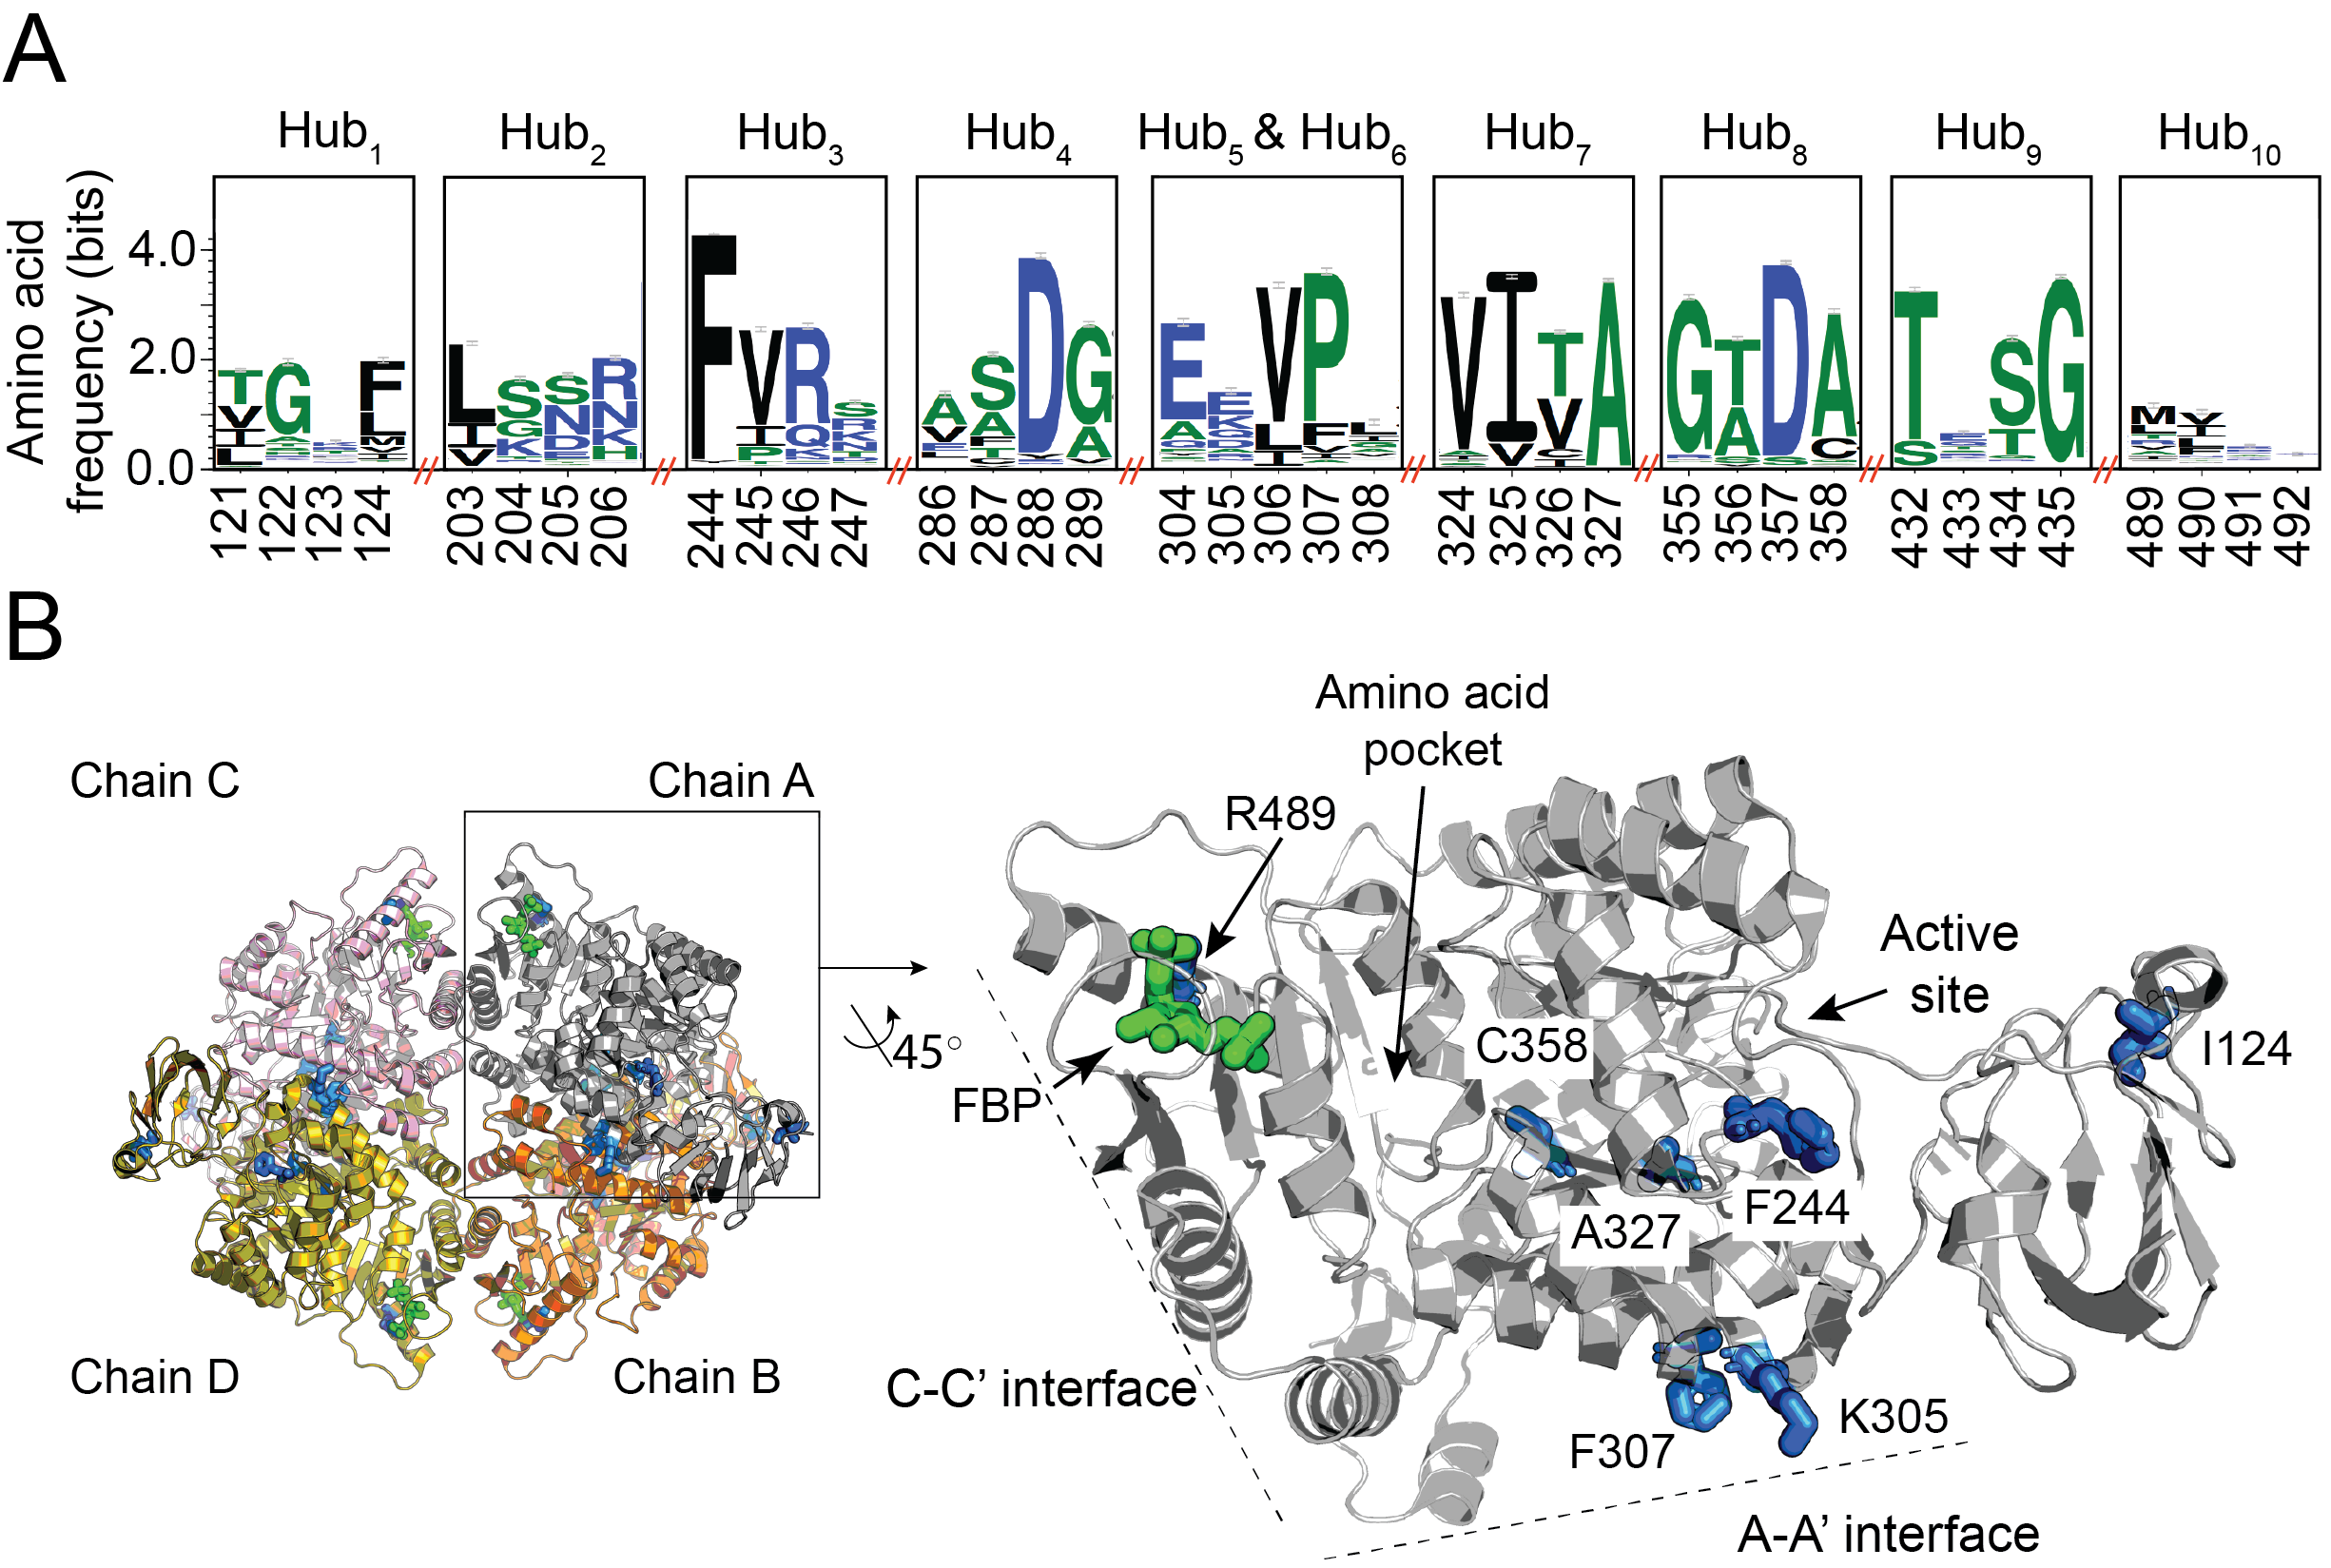
\includegraphics[scale=0.7]{ch6_fig14_allohubfrag_sequence.png}
\caption[Design of Allosteric Hub Mutants (AlloHubMuts).]{\textbf{Design of Allosteric Hub Mutants (AlloHubMuts).} Allosteric Hub Mutants (AlloHubMuts) were designed based on an empirical prediction of which residues would be tolerated at each AlloHubFrag position. \textbf{(A)} A logo-plot of the AlloHubFrags from a multiple sequence alignment of 5381 pyruvate kinase homologues. \textbf{(B)} The residue positions of the AlloHubMuts.}
\label{fig:allohub_design}
\end{figure}

\clearpage

\section{Conclusion}
Ion-mobility coupled to mass spectrometry measurements in Chapter \ref{chapter:mass_spec} revealed that PKM2 undergoes conformational changes upon FBP binding, though the molecular details of the conformational changes were elusive. To this end, we performed an extensive characterisation of the conformational dynamics of PKM2 bound to various allosteric ligands. MD simulations of monomeric and tetrameric PKM2 found that allosteric activator binding induces the closure of the B-domain over the catalytic pocket. The ligand-dependent dynamics of the B-domain is therefore proposed as a determinant of enzyme activation, which traps highly resident water molecules proximal to the substrate binding pocket. 
%
%
\\\\
%
%
A computational method \textit{AlloHubMat} was developed and applied towards identifying allosteric hub residues, which orchestrate the transmission of allosteric information between ligand binding pockets and the active site. We found a network of allosteric hub residues, which are predicted to potentiate the effects of FBP allosteric within PKM2. The AlloHubFrags were used as a template to design a collection of single-point mutant variants (AlloHubMuts) of PKM2, to test the hypothesis that these residues are involved in the allosteric mechanism of the protein.







